\documentclass{classes/sysuthesis}
\usepackage{multirow}


%%
% 论文相关信息
% 本文档中前缀"c-"代表中文版字段, 前缀"e-"代表英文版字段

% 标题
%论文题目:在 25字以内,能简明、具体、确切地表达论文特 定内容,必要时,可以使用副标题。中文、英文题目应一致。


% 中英文标题
\ctitle{面向多样场景的鲁棒单目深度估计算法研究}
\etitle{Research of Robust Monocular Depth Estimation for Various Scenes}

% 作者详细信息
\cauthor{潘孟}    % 作者中文名
\eauthor{Meng Pan}	%作者英文名
\degree{硕士}		%硕士or博士
\studentid{18215490}	%学号
\cschool{智能工程学院}	%学院

\cmajor{检测技术与自动化装置}	%专业名称
\emajor{Detection Technology and Automatic Equipment}	%英文专业名称

% 指导教师
\cmentor{金枝 副教授}
\ementor{Asoc. Prof. Zhi Jin}

     % 论文相关信息
%%
% 摘要信息
% 摘要内容应概括地反映出本论文的主要内容,主要说明本论文的研究目的、内容、方法、成果和结论。要突出本论文的创造性成果或新见解,不要与引言相 混淆。语言力求精练、准确,以 300—500 字为宜。
% 关键词是供检索用的主题词条,应采用能覆盖论文主要内容的通用技术词条(参照相应的技术术语 标准)。按词条的外延层次排列(外延大的排在前面)。


\cabstract{
	摘要概括论文的主要信息,包括研究目的、方法、成果及 最终结论。硕士论文摘要一般不超过 1200字。博士论文摘要 一般不超过 2000字。关键词是供检索用的主题词条,应采用 能覆盖论文主要内容的通用词。关键词一般列 $3-5$个。
}
% 中文关键词(每个关键词之间用“;”分开,最后一个关键词不打标点符号。)
\ckeywords{研究目的;研究方法;创新性成果;独特见解 }

\eabstract{
	Image color editing is one of the most generous image processing tasks, which borrows one image’s color characteristics to another so that the color appearance of these two images are visually similar. This is a process to change image color style to another specified style. Color editing techniques can adjust the image's color and its artistic style,according to the needs of different applications, e.g. film production, photo processing and web design. The key problem is how to achieve a satisfied color editing result and preserve the contents of the source image well. 
	
	In this paper, we discover many edge-aware smooth methods and non-linear color mapping based color transfer methods in literature. Combined with geometric target region extraction and correction operation, we present two methods to achieve visually satisfied interactive edge-aware image color editing results. One is color distribution mapping based on multi-scale gradient-aware decomposition, and the other is interactive image color transfer based on multi-cue manipulation. The color distribution mapping decomposes the image editing issue into image color edge preservation and color transfer. First, input image is decomposed into multiple detail layers and base layers using edge-preserving WLS operator. 
}
% 英文文关键词(关键词之间用逗号隔开,最后一个关键词不打标点符号。)
\ekeywords{Image Editing, Edge Preserving, Color Mapping, Color Clustering, Image Inpainting}     % 摘要内容

\begin{document}
    % 论文前置部分
    \frontmatter
        \pagenumbering{Roman}
        \maketitle    % 扉页
        \makedisclaim       % 原创性及学位论文使用授权声明 
         
	    \makeabstract       % 中英文摘要
        \maketableofcontents        % 目录
        
        %缩略语
        %%列举文章中出现的专业名词缩略语对应的中文全称和英文全称,注意按首字母顺序排序

\chapter{\heiti{缩略语}}
\begin{longtable}{p{2.5cm}p{8cm}p{5cm}}
	\heiti{缩略语}		&\heiti{英文全称}														 	&\heiti{中文全称}        \\
	3GPP 					& 3rd Generation Partnership Project 					& 第三代合作伙伴计划                                  \\
	OFDM  					& Orthogonal Frequency Division Multiplex  	  & 正交频分复用                        \\	
	V2V 						& Vehicle-to-Vehicle  & 车联网                                     \\														
\end{longtable}
        %\newclearpage
        
        %数学符号
        %%列举文章中出现的数学符号及其含义

\chapter{\heiti{数学符号}}
\begin{longtable}{p{4.0cm}p{11.0cm}}
	\heiti{符号}				 &\heiti{含义}														 	       \\
	$(\cdot)$ 					& 矩阵的共轭转置  	                          \\	
	$ \|\cdot\|_F$			& Frobenius范数                                      \\														
\end{longtable}
        %\newclearpage

    % 论文主体部分
    \mainmatter
        % 引言

        % 正文
        \chapter{引言}
%引言是论文正文的开端,应包括毕业论文选题的背景、目的和意义;
%对国内外研究现状和相关领域中已有的研究成果的简要评述;
%介绍本项研究工作研究设想、研究方法或实验设计、理论依据或实验基础;
%涉及范围和预期结果等。要求言简意赅,注意不要与摘要雷同或成为摘要的注解。
\label{cha:introduction}
\section{选题背景与意义}
\label{sec:background}
近年来,人工智能技术快速发展,日新月异。复杂多变的环境对人工智能技术
提出了更高的要求,更加智能的算法成为了人们的追求。
从周围环境中获取准确信息是智能体对周围环境做出决策的基础,其中深度估计,
即获得环境与智能体之间的距离信息,对于智能体来说十分重要。
尤其对三维重建,3D物体检测,即时定位与建图等任务更是不可或缺的步骤。
在深度估计算法中,传感器感知算法使用传感器依靠环境对自身释放信号
的反馈来获取信息,例如通过雷达扫描获得点云数据进而预测深度。
其优点是较为精确,算法稳定不易受到环境干扰。但是存在数据稀疏,
设备成本高的问题。广泛使用的还有双目立体匹配算法,模拟了生物的双眼,
通过对双目相机获取的图像进行立体匹配,从而获得双目视差信息,进一步依靠基线
和几何知识可获得深度信息。但是,双目相机完全同步较为困难,
且对硬件条件(相机相对位置,绝对位置,
相机内参外参等)要求较为严格。
单目深度估计即从一张给定的RGB图像中恢复出图像中的场景到
相机的距离,并存储在深度图像素中。该问题可以被描述为:
给定一个集合$\mathcal{T} = \{(I,D)\}$, 
$I\in \mathcal{I}$, $D\in \mathcal{D}$,
其中$\mathcal{I}$和$\mathcal{D}$分别是RGB图像和真实深度图集合,
算法希望获得从$\mathcal{I}$到$\mathcal{D}$的映射
$\varPhi : \mathcal{I} \rightarrow \mathcal{D}$. 

单目深度估计算法相比传感器和双目深度估计具有独特的的优势:
对硬件要求较低,
采集单目RGB图像的相机可以是消费级。
基于这些优势,近年来学者们对单目深度估计算法进行了深入的研究。
但是单目深度估计算法也有其不可忽视的缺点:
场景的3D信息在图像采集过程中完全丢失,因此,要恢复已损失的深度信息,
算法需要拟合的映射$\varPhi$缺乏理论依据,
这使得算法实现具有一定难度。但是随着深度学习技术的不断进步,
数据在多样性和数量上得到了极大的丰富,计算能力大幅提高。
在这些技术的支撑下,通过真实信号的引导使得神经网络“学习”这
个无规则的映射成为了可能。

\section{国内外研究现状和相关工作}
深度信息的获取是多领域的研究热点,
近年来学者们针对如何获得深度信息开展了一系列的研究,在方式上可分为
传感器法,几何约束法,深度学习法。本章主要介绍深度估计的研究现状和
相关工作,从三个方面分别进行介绍,重点介绍了深度学习方法。


\subsection{传感器法}
深度传感器法\cite{zhang2012microsoft,yoneda2014lidar}
能够直接获取相应图像的深度信息。RGB-D相机具有直接获取RGB图像
像素级密集深度图的能力,但受测量范围和室外阳光敏感度的限制。
虽然激光雷达被广泛应用用于无人驾驶行业的深度测量,
但是只能生成稀疏的三维地图。此外,这些深度传感器
(RGBD相机和LIDAR)的尺寸和能耗影响了它们在小型机器人
如无人机中的应用。由于单目摄像机具有成本低、体积小、
应用范围广等特点,基于单目图像的密集深度图估计方法受到了越来越多的关注,
近年来基于端到端深度学习的方法得到了广泛的研究。
\subsection{几何约束法}
使用多张图像构成几何约束法
\cite{zou2010method,cao2015summary,ullman1979interpretation}
来恢复三维信息近年来被学者广泛研究。从运动估计结构(
Structure From Motion, SFM)\cite{ullman1979interpretation}
是几何约束法的代表性方法。
深度信息可以通过图像序列之间的特征匹配和几何约束来估计,
即深度估计的精度在很大程度上依赖于精确的特征匹配和高质量的图像序列。
此外,SFM还存在尺度模糊问题。立体视觉匹配还能够通过从两个
视点观察场景来恢复场景的3D结构,通过两个摄像机模拟人眼的视觉方式,
通过代价函数计算图像的视差图。
与基于单目序列的SfM方法不同的是,在立体视觉匹配过程中,
由于两个摄像机之间的距离是预先标定的,所以深度估计中包含了尺度信息。
上述基于几何的方法可以有效地计算稀疏点的深度值,但这
些方法通常依赖于图像对或图像序列。由于缺乏有效的几何解,
如何从一幅图像中提取出稠密的深度图仍然是一个重大的挑战。
\subsection{深度学习法}
从图像中估计深度信息是计算机视觉领域重要的任务,在即时定位与建图
(SLAM),自动驾驶,物体检测等诸多任务中有着广泛的应用。
在研究过程中先后经历了几何算法、手动提取特征结合神经网络算法,
有监督学习方法、无监督学习方法和半监督学习方法几个过程。本章将围绕
基于深度学习的单目深度估计算法的发展经历展开叙述。

\subsubsection{手动提取特征}
以前的工作通常侧重于利用几何先验知识或其他信息源,
大多数使用手工制作的特征。
Saxena等人\cite{saxena2006learning}创造性地
将深度学习应用在单目深度估计中。该方法首先收集一组
非结构化的户外环境单目图像,例如森林、树木、建筑物等及其相应的真实
深度图。然后手动提取了一系列特征,并使用马尔可夫随机场(MRF),
结合多尺度的局部和全局图像特征,对单个点的深度
以及不同点深度之间的关系进行了建模。

Saxena等人\cite{saxena2007}随后对以上方法进行了改进。
该方法应用马尔可夫随机场(MRF)学习算法来捕捉这些单眼线索,
并将它们整合到一个双目立体系统中。实验结果表明通过将单目线
索添加到双目立体测距系统中,可以获得比单独使用单目或双目立体
更精确的深度估计。
\subsubsection{有监督方法}
传统的机器学习方法来进行单目深度预测存在着人为先验假设较多,
不能端到端的处理使得整个过程过于复杂等缺点,这些缺点对更加
标准,流程统一化的
网络提出了需求。随着数据在多样性和数量上的极大丰富,以及
计算能力的高速增长,深度学习技术迅速发展。神经网络
在计算机视觉、控制工程、多媒体、自然语言处理等领域显示了其
强大的优势。

%使用深度学习算法处理深度估计问题根据不同的标准可以
%大致分为以下四类:
%1) 有监督方法/半监督方法/无监督方法
%2) 绝对深度引导/相对深度引导
%3) 单任务/多任务
%4) 回归模型/分类模型

有监督深度学习方法需要真实的深度图来引导整个训
练过程,所以单目深度估计
可以建模为一种回归问题。
最常见的损失函数为$\mathcal{L}_2$ loss:
\begin{align}
    \mathcal{L}_2(d,d^*) = 
    \frac{1}{N} \sum\limits_{i}^{N} \|d-d^*\|_2^2   
\end{align}
其中$d$与$d^*$分别为预测深度值与真实深度值,$N$为图像像素数目。
Eigen等人 \cite{eigen2014depth} 
首先设计了一种端到端的单目深度估计网络,
网络使用两个
级联的子网络来进行预测。一级网络重建了较粗粒度的深度图,尺寸为
原图像尺寸的1/4,该深度图随后被送入精细重建子网络,恢复出
细节更加精细的深度图。同时论文提出了一种新的尺度不变性损失函数:
\begin{align}
\mathcal{L}_{scale-invariant} = 
\frac{1}{N} \sum\limits_{i}^{N} y_i -\frac{1}{N^2} 
(\sum\limits_{i}^{N} y_i)^2
\end{align}
其中$y_i = |d-d^*|$。该团队随后
改进了这一网络\cite{eigenthreetasks},同时完成了
深度预测、法线预测、语义分割三个任务。该网络较\cite{eigen2014depth}
使用了更深的骨干网络VGGNet\cite{vgg},
同时增加了第三个用来提高重建尺度的网络,使得重建图像为
原图的1/2,最后前两个尺度网络从输出一张重建图变为输出多通道的特征图。

Liu等人\cite{liu2015learning}考虑到深度值的连续性,
深度估计可以自然地表示为一个连续条件随机场(Continuous CRF)学习问题。
联合卷积神经网络和连续条件随机场提出了一种
用于单目图像深度估计的深度卷积神经场模型。这是一种更深层结构的学习架构,
在一个统一的深层神经网络框架下学习连续CRF的一元势能项和成对势能项。
在此基础上,进一步提出了一种基于完全卷积网络的等效模型和一
种新的超像素池化层方法,使得处理速度提高10倍左右。

Li等人\cite{li2015depth}通过对深度卷积神经网络特征的回归,
结合条件随机场(CRF)的后处理细化步骤来解决单目深度估计问题。
论文从超像素级和像素级两个层面进行重建。首先设计了
一个深度神经网络模型来学习从多尺度图像块到超像素水平的深度
和表面法线值的映射。然后通过优化
超像素尺度的一元势能、成对势能以及像素尺度的自回归势能,
将估计的超像素深度和表面法线细化到像素级。
该方法在Make3D和NYU depth v2数据集上的实验取得了在当时
具有竞争力的结果。

Laina等人\cite{laina2016deeper}设计了这一种带有残差网络的全卷积
网络作为基础网络进行深度估计。为了提高分辨率,该团队提出了一个有效的学习网络
中特征的上采样方法,在设计完基础结构部分,对基础细节结
构做了改进。在传统上采样结构中,存在uppooling的结构,
这种方式得到的结果中很多0值,这
让网络进行了很多的无效运算,降低了效率,该方法采用了小卷积的方式,
使用了四种小卷积核,这四种小卷积核恰好能够包含原有的5$\times$5
卷积核的所有部分。
卷积得到的结果可以大量减少0的出现。在拼接的时候记录了每个
特征图上的位置,根据位置再上采样。这种结构可以
大大降低无效运算,提高运行效率。同时提出了Huber loss 作为损失函数:
\begin{align}
    \mathcal{L}_{Huber} = 
    \begin{cases}
        |x| & \text{$ |x| \leq c$} \\
        \frac{x^2+c^2}{2c} & \text{$|x| > c$}
    \end{cases}
\end{align}其中$x = d_i - d_i^*$.
当误差在C范围内为$|X|$就退化成了L1范式,而当超过C时就则退化为L2范式。
Huber loss 对两种损失都有了一种平衡。

以上方法均为通过绝对深度信息来引导神经网络的拟合,但是在实际场景中
人们有时候会通过确定的深度信息来推测其他物体的深度信息。
即依靠相对深度关系来推测深度。
学者们随后开始使用物体或者场景之间的相对深度关系来完成
深度估计。

首先关注到深度相对关系的是Zoran\cite{zoran2015learning}。
该方法对输入图像中的点进行
两两相对关系估计。将这些稀疏的相对关系深度图基于全局进行度量来
创建连续度的深度图。估计点与点之间的相对
关系比直接度量估计有几个优点:它比暴力回归更加简单,另外人类
更擅长相对判断,因此数据收集更容易;
最重要的是这种相对顺序关系对数据具有单调变换不变性,
从而提高系统的鲁棒性。
方法首先使用神经网络提取有序点对,然后再估计点对之间的深度关系。
同时该方法证明了这个框架在图像内部分解和深度估计
两个重要的任务上都能很好地工作。

Chen等人\cite{chen2016}提出了第一个相对深度数据集: Depth in the Wild。
它由49.5万张不同的图像组成,每张图像都有随机取样点及其相对深度的注释。
文章还提出了一种新的使用相对深度来估计深度的方法,
与Zoran\cite{zoran2015learning}相比更加简单且表现更好。
该方法由一个直接预测像素深度的单一深度网络组成。网络以整个
图像作为输入,由沙漏网络组件组成,可以通过相对深度的标注进行训练。
方法具有两个优点:(1)多尺度深度网络,产生像素级的度量深度预测;
(2)使用了相对深度的损失函数Ranking loss:
\begin{align}
    L(I,R,z) = \sum\limits_{k=1}^{K} \psi_k (I,i_k,j_k,r,z)
\end{align}
设计相对深度损失函数的目的是使得输出的深度预测图中的关键点
能够满足真实
的前后顺序关系。考虑一张训练图片$I$具有$K$个关键点,
$r_k \in \{+1,-1,0\}$代表$i,j$两点真实的相对深度关系,
如果i点比j点近,则$r$为1,否则为-1,距离相近则为0。$z$为网络
预测深度。此损失函数的设计,让网络能够利用相对深度关系作
为标签,网络直接输出深度值。

一部分学者发现深度信息与其他信息具有很高的相关性,例如语义信息,
边缘信息,法线信息等。于是出现了许多多任务联合框架来解决
深度估计问题。

基于语义分割与深度信息的互补性,Wang等人\cite{2015semantic}
提出了一个深度和语义双任务联合预测框架。
给定一幅图像,首先使用一个预训练的卷积神经网络来预测深度图和语义图。
通过深度和语义信息之间的互补特性,联合网络提高了单一任务深度预测或者
语义分割的精度。为了进一步重建精细的层次细节,
在全局信息指导下,对图像进行局部分割,随后构造了两层级联条件随机场
(Hierarchical CRF)
以加强全局和局部预测之间的协同作用,
其中全局信息用于指导局部预测和减少局部模糊,而局部结果提供
了详细的区域结构和边界。这篇文章通过广泛的实验,证明了
使用联合框架解决深度预测和语义分割对两个子任务的指标均有
很大的提升。

Mousavian等人\cite{2016semantic}同样将语义分割和深度预测理解为
像素映射到标签的问题。该方法首先使用一组权重相同的特征提取器来提取特征,
这些特征随后在每个尺度都被送往两个神经网络进行计算,一个用来预测深度,
一个用来进行语义分割。随后每个尺度的特征图在通道维度进行连接,
预测出最终深度图。深度图随后被加入到全连接随机场(Fully Connected CRF)
来预测最后的语义结果。

以上方法均将单目深度估计建模为一种回归问题,由于深度图中每个像素
存储了深度信息,所以该问题可以被建模为像素分类问题。
Cao等人\cite{cao2017estimating}利用深度残差网络 (ResNet)
提出了一个像素级的分类网络。该方法首先将连续的深度值离散
成多个标签,然后深度残差网络来预测每个像素的深度标签。
使用离散深度标签分类代替连续深度值回归,可以预测像素在
每个深度标签的置信度。进一步应用全连接条件随机场
来对局部细节进行后处理,从而改进了结果。
\subsubsection{无监督方法}

有监督方法需要真实标签来引导训练过程,但是获取稠密的真实深度图是个复杂的问题。
雷达点云数据精度高,但是只能获取稀疏点云。深度相机获取的深度图
较点云相对稠密,但是仍有很多的空洞。这在监督训练时对预处理提出了
更多的要求。无监督训练,即对训练过程添加隐式的约束,从而舍弃掉对
标注的依赖解决了稠密深度图难以获取的问题。

Garg等人\cite{garg2016unsupervised}首次提出了一种无监督框架。
该方法需要双目图像作为输入,首先左图像通过一个卷积神经网络(CNN)输出
一张深度图,随后将深度图转化为视差信息,利用视差信息右图像可以
合成出一张‘左视图’,利用左视图和合成左视图的光度误差信息来使合成图像
趋近于左图像,受到左右视图一致性的约束,整个训练过程得以在没有
真实深度的情况下使CNN学习到RGB图像到深度图的映射。
\begin{figure}[htb]
    \centering
    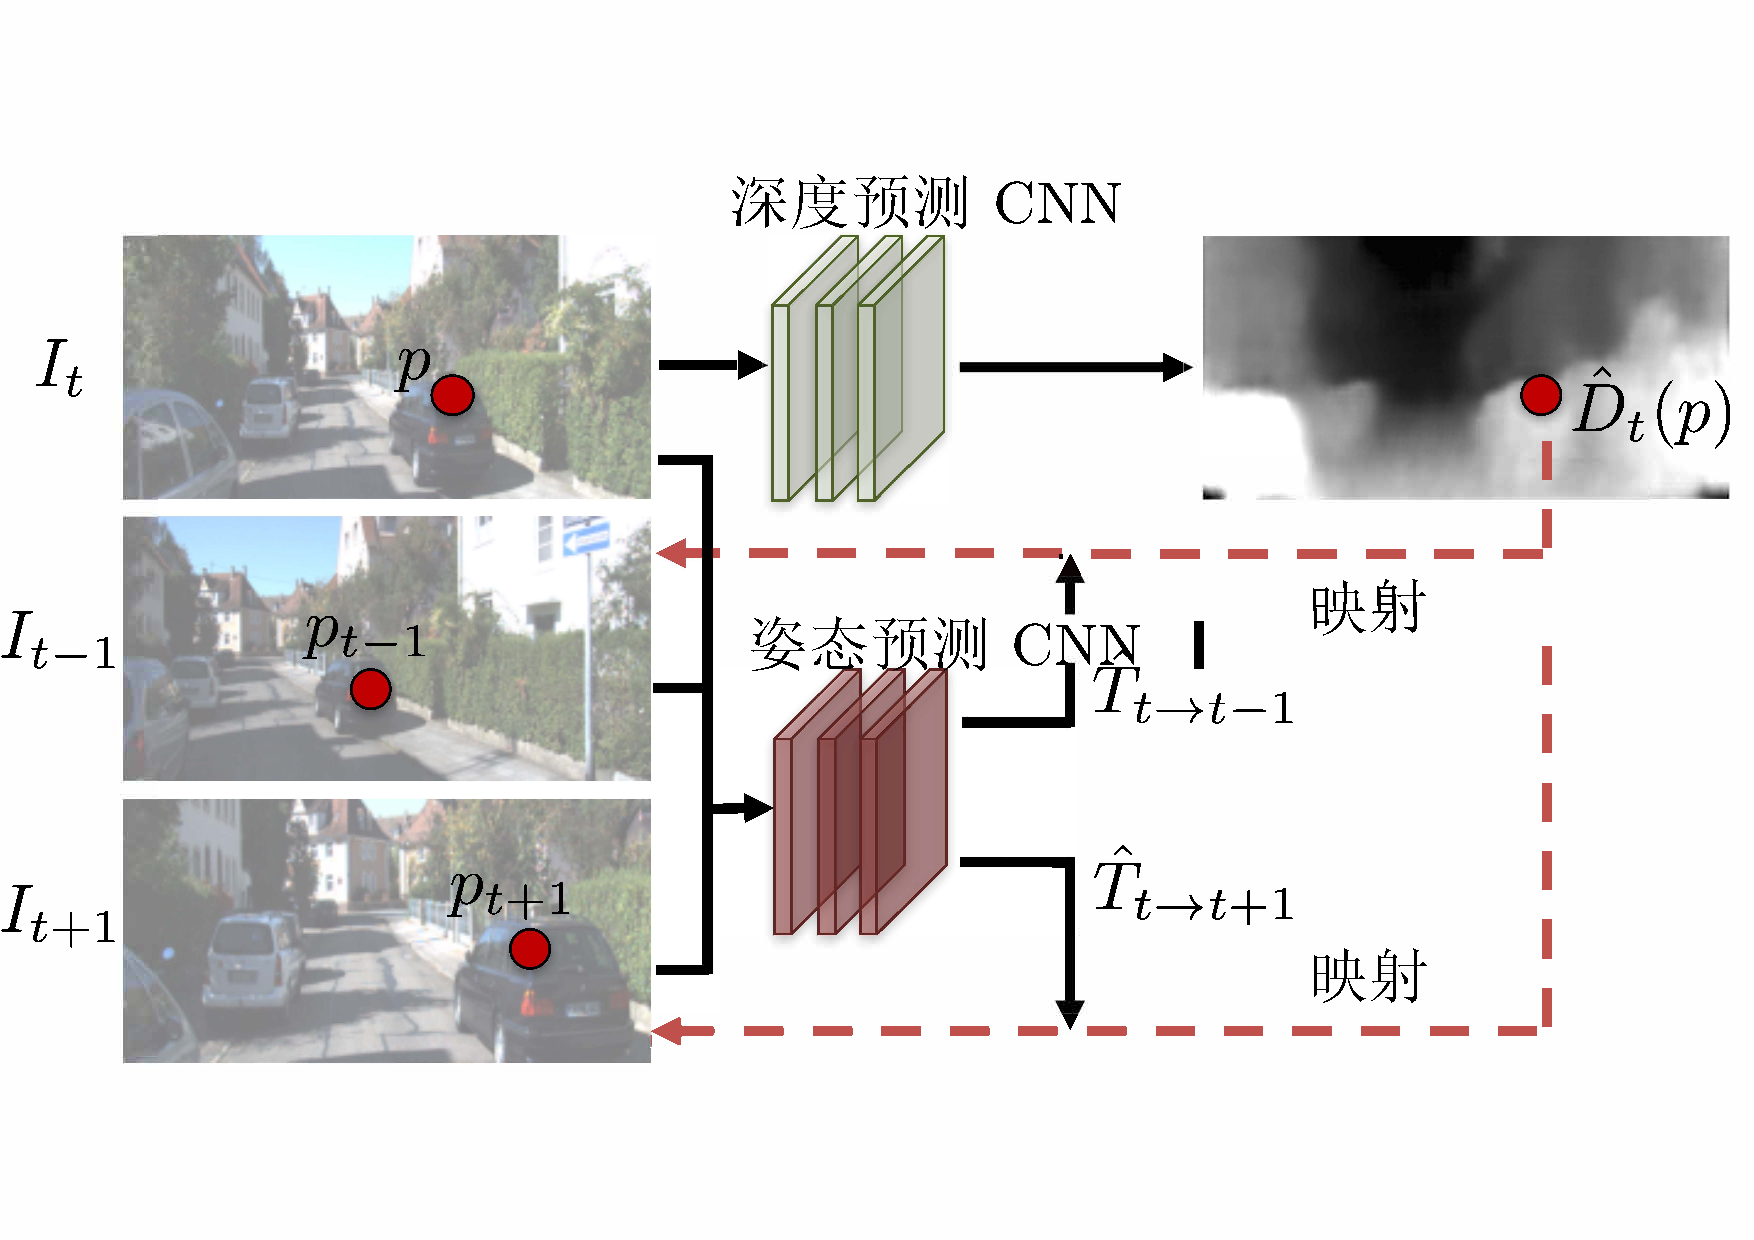
\includegraphics[width=0.9\linewidth]{figure/Sfm.pdf}
    \caption{Zhou等人\cite{zhou2017unsupervised}提出的无监督
    训练框架,可以同时预测相机姿态与深度信息。}
    \label{sfm_zhou}
\end{figure}

Zhou等人\cite{zhou2017unsupervised}提出了一种姿态和深度联合估计的
框架。这种框架利用一段视频作为输入,以视频中的三帧图像为例,
方法使用一个神经网络对中间帧进行深度估计,同时以中间帧和前帧作为
姿态网络的输入,得到一个六自由度的姿态转换矩阵,当获得姿态和深度信息后
中间帧可以重新合成出一张前帧,利用前帧与合成前帧的光度误差,可以
约束整个训练过程,后帧同理。该方法不仅可以同时进行相机的姿态估
计和深度估计,而且不需要任何的数据标注,只需要一段视频即可完成。
在视觉里程估计(VO)和即时定位与建图(SLAM)方向都有很重要的意义。

双目无监督估计\cite{garg2016unsupervised}存在着一些问题:
双目图像并不是完全相同的,左视图和右视图分别有一些各自的盲区;
另外还有遮挡移动等问题会影响预测的结果。
所以针对这些问题Godard等人\cite{Godard2019}提出了一种解决方法:
针对移动和遮挡的问题,设计了一种掩码,
该掩码解决了假设相机在静态场景中移动变化有关的问题。尤其是
一个物体正在以与相机相似的速度移动,
也就是那些在相机坐标系里静
止的物体。这些相对静止的物体的位置在无监督算法的前后帧
几乎没有变化,也即视差为0,理论上应该有无穷大的深度。该
方掩码可以过滤从一帧更改为下一帧时造成误差的像素,
即那些和相机同步运动的像素。
\begin{figure}[tbp]
    \centering
    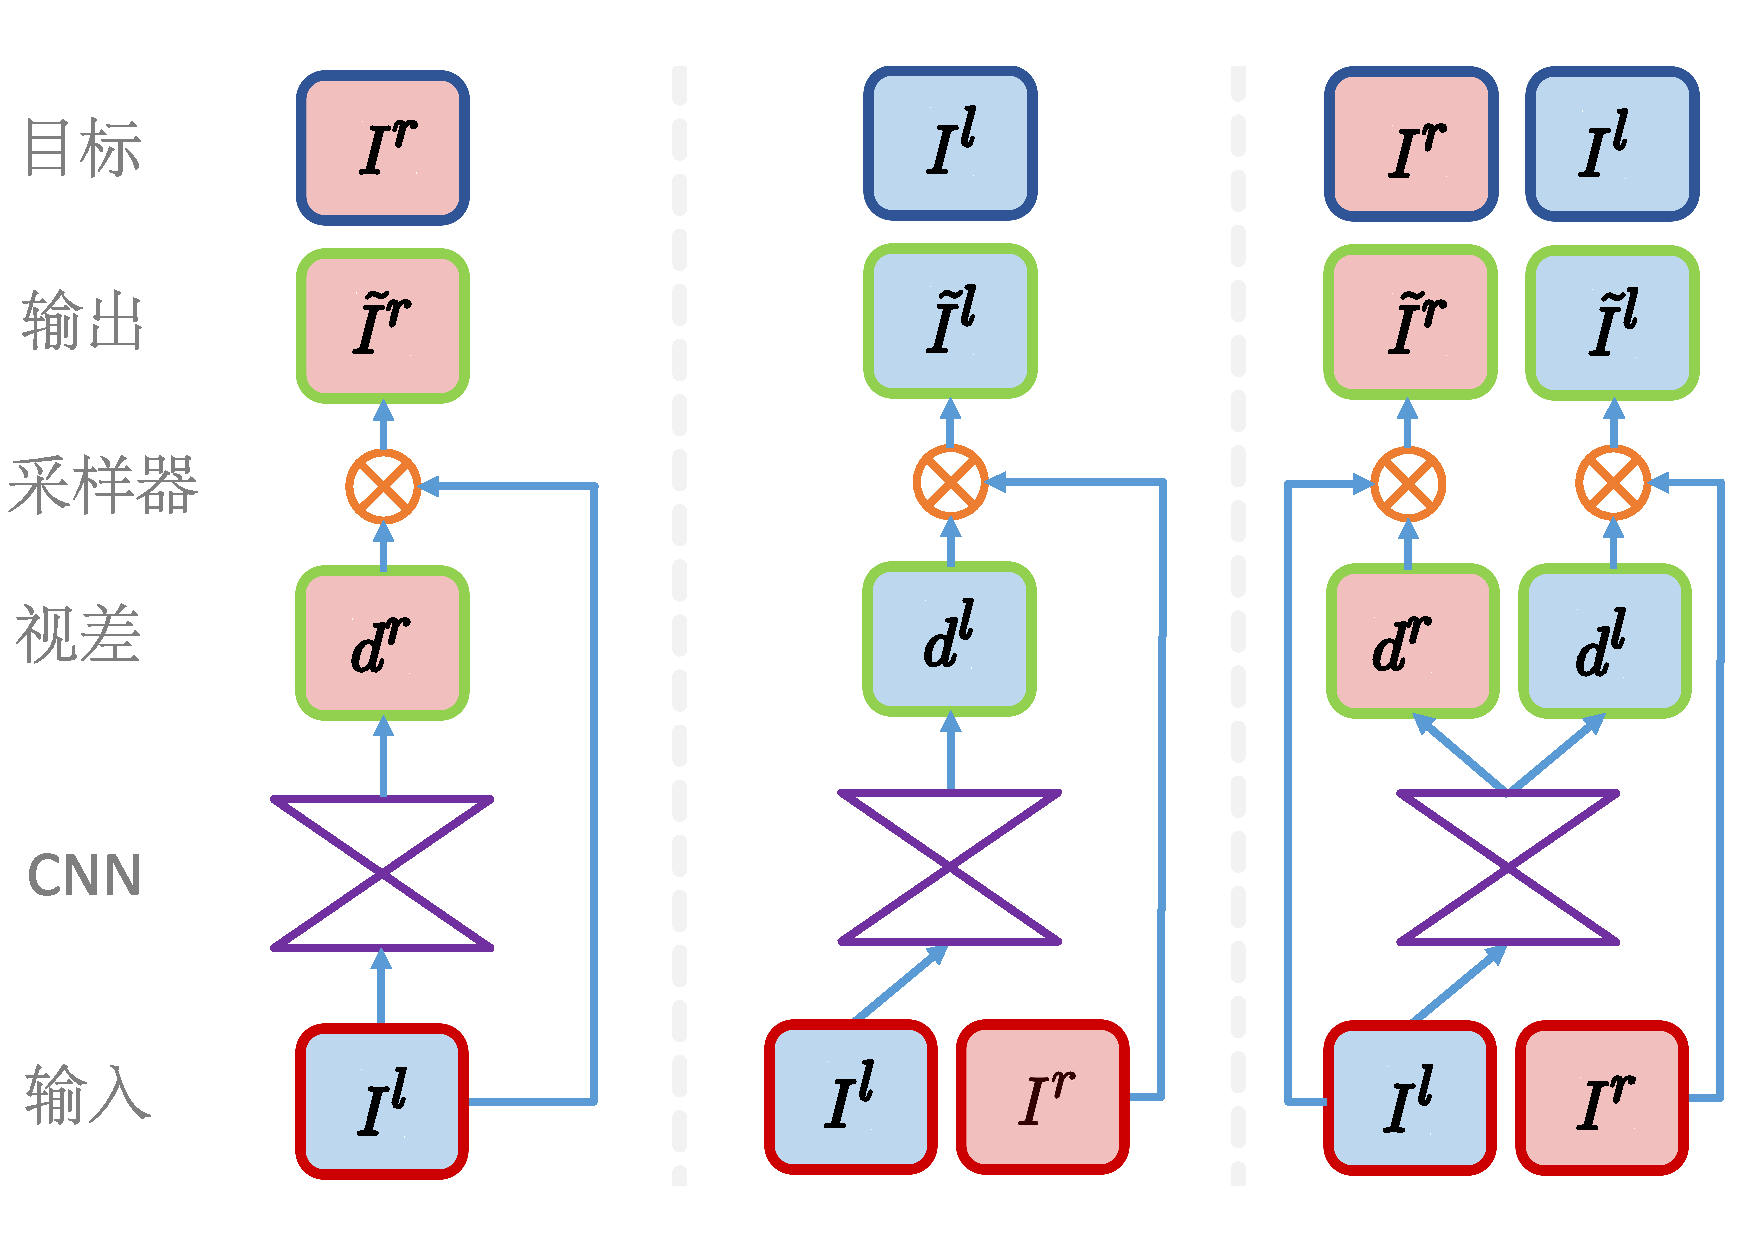
\includegraphics[width=0.7\linewidth]{figure/lr.pdf}
    \caption{Godard等人\cite{Godard2019}根据左右视图的一致性,提出了
    双目无监督框架。}
    \label{Sfm}
\end{figure}
\subsubsection{半监督方法}
%两级标题之间要有过渡性文字。可以通过一段话引出下面的文字
%或者对本章内容概括。论文中凡非正式参考文献以外的资料,
%应以脚注的方式注明\footnote{大家要养成添加脚注的好习惯}。
由于不需要标注数据,无监督方法的性能与有监督方法还有一定的差距。
另外,无监督方法也存在各种各样的问题,例如尺度不一致问题等。
因此,学者们在减少对标注数据的依赖下提出了一种提高估计精度的半监督方法。

Kuznietsov等人\cite{kuznietsov}提出了一种依靠双目图像和雷达点云
数据的半监督预测框架。该框架需要一组双目RGB图像和对应的雷达点云
作为输入。双目图像经过CNN后预测出一对深度图,深度图与稀疏的点云数据在
监督损失函数的约束下趋于一致。同时深度图可以与双目视图中的一张图像
合成出另一视角的观测图像,该图像在无监督损失函数的作用下与
真实的图像趋于一致。
除了这两个损失函数,作者还根据深度图只在物体边缘发生
剧变的特性设计了梯度平滑损失函数。

\section{本文的研究内容与主要工作}

本文的创新点及主要工作如下:
\begin{enumerate}
    \item 针对单目深度估计任务提出了一种基于像素分类的单目深度估计
    框架。该框架在像素级别上生成一系列的备选深度,预测该
    像素上每个备选深度的置信度,如图\ref{Pick}所示。
    \begin{figure*}[htb]
        \centering
        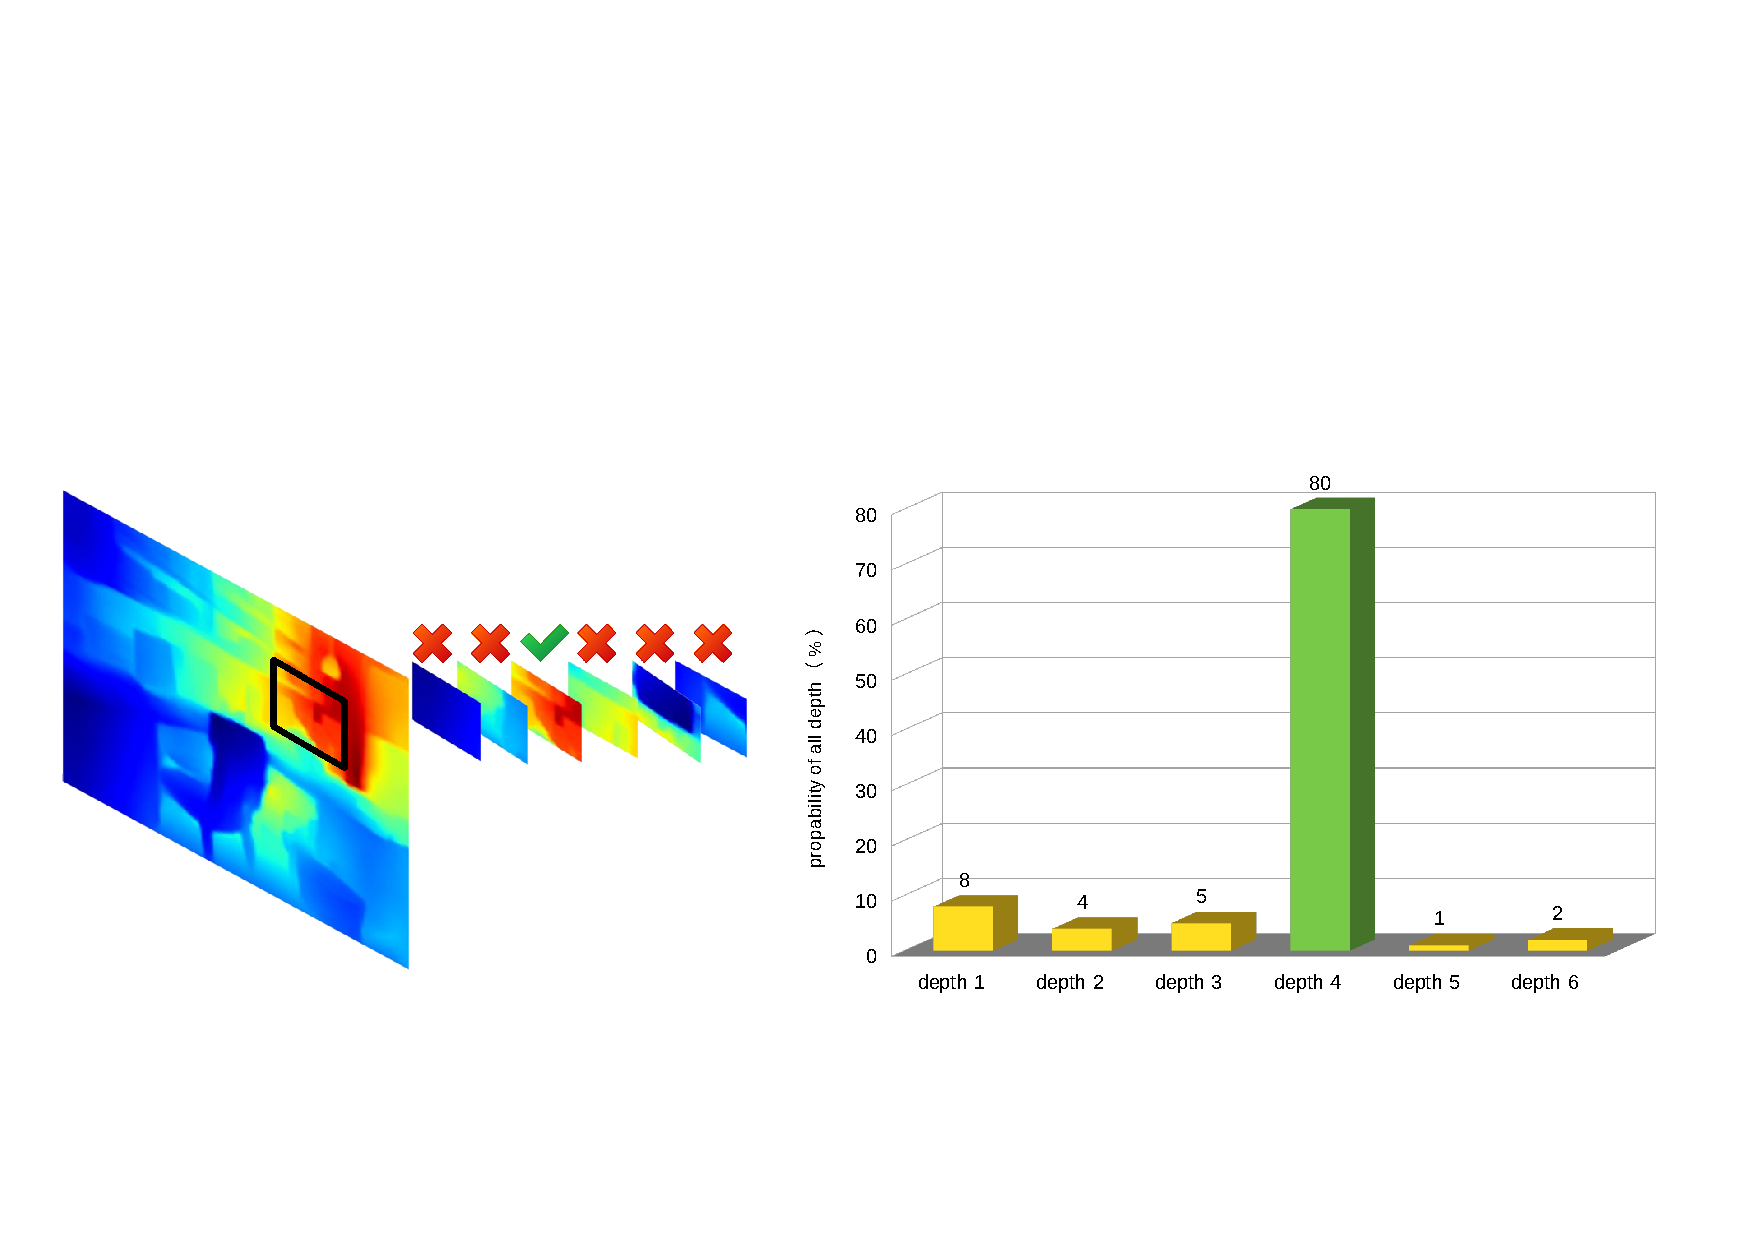
\includegraphics[width=0.9\linewidth]{figure/Pick.pdf}
        \caption{在每个像素位置生成一系列备选像素并计算每个深度的置信度}
        \label{Pick}
    \end{figure*}
    在上采样结构中加入了特征注意力模块(Feature Attention Module),
    该模块在上采样过程中,将短路连接输入的编码端特征图与解码端特征图
    在通道维度内做了不同程度的关注,使得两个信息源有所侧重的重建深度。
    \item 现有算法大多在单一场景进行实验,例如在室外场景数据集训练并且测试,
    或者在单一的室内场景数据集训练和测试。这种算法鲁棒性较差:
    当将室外场景数据集训练的算法应用在室内数据集时表现不佳。
    本文旨在提高算法的泛化能力,
    创造性地将室外数据集合室内数据集结合在一起对单目深度估计进行训练。
    但是预测结果相比单一数据集出现了退化现象。即复杂多样的数据集对
    网络拟合能力和表达能力带来的挑战。
    \item 为了进一步提高网络的拟合能力和表达能力,受到知识蒸馏算法的启发,
    本文提出了一种自蒸馏单目深度估计框架。
    经过实验对比发现,该自蒸馏方法可以有效地解决网络在面临多种数据
    分布时的退化问题。大大提高了网络的表达能力与拟合能力。
    更重要的是该的框架可以应用于所有的端到端编解码网络,
    为后面的融合工作打下了基础。
\end{enumerate}

\section{本文的论文结构与章节安排}

\label{sec:arrangement}
本文共分为五章,各章节内容安排如下:第一章介绍了选题的背景和意义,
按照类别介绍了国内外在单目深度估计的发展现状。并简要描述了
本文的创新点以及工作。因为本文以深度学习算法为基础来进行算法
实现,所以在第二章深度学习算法概述中重点描述本文
使用的卷积神经网络(CNN),以及基于深度学习的单目深度估计
的基础知识:例如常用数据集和评价指标等。
第三章描述了本文提出的基于像素分类单目深度估计方法,该方法是端到端的编解码网络,
在编码端添加了向解码端输入数据的短路连接。在解码端设计了
特征注意力模块,用来对编码端输入的特征和解码端的特征进行
有效地关注,从而提升重建效果。
第四章介绍了提出的自蒸馏学习框架,并进行了实验验证,实验表明
该框架可以有效地解决网络面对复杂数据集的表达能力不足,难以
拟合的问题。
第五章对本文总结反思,审视不足,展望未来工作。


        \newclearpage
        \chapter{梯度感知的颜色分布映射方法}
本章内容概括。
\section{图像颜色编辑的梯度感知优化策略}
论文主体是毕业论文的主要部分,必须言之成理,论据可靠 \cite{tighe2013finding},严格遵循本学科国际通行的学术规范。在写作上要注意结构合理、层次分明、重点突出。

本章举例说明本模板中图片,表格及公式的插入及引用方法 \cite{liu2011sift}。

\subsection{图片格式举例}

图片的分辨率至少300个像素,建议格式为.png或.eps。图 \ref{fig1} 显示……,图 \ref{subfig1} 表明……。

\subsubsection{单张图片}
\begin{figure}[h]
	\centering
	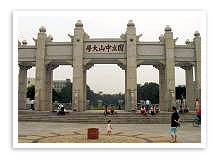
\includegraphics[width=0.8\textwidth]{figure/fig1.png}
	\caption{标题} 
	\label{fig1}
\end{figure}

\subsubsection{多张子图}
\begin{figure}[h!] % image examples & compare
	\begin{subfigure}{0.55\textwidth}
		\centering
		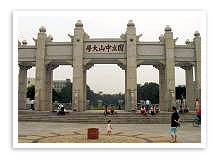
\includegraphics[width=0.5\textwidth]{figure/fig1.png}
		\caption{子图1}
		\label{subfig1}
	\end{subfigure}
	\begin{subfigure}{0.55\textwidth}
		\centering
		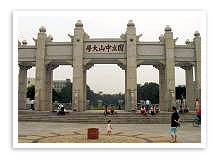
\includegraphics[width=0.5\textwidth]{figure/fig1.png} 
		\caption{子图2}
		\label{subfig2}
	\end{subfigure}
	\begin{subfigure}{0.55\textwidth}
		\centering
		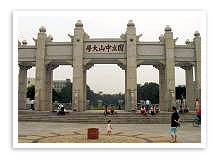
\includegraphics[width=0.5\textwidth]{figure/fig1.png}
		\caption{子图3}
		\label{subfig3}
	\end{subfigure}
	\begin{subfigure}{0.55\textwidth}
		\centering
		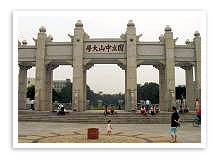
\includegraphics[width=0.5\textwidth]{figure/fig1.png} 
		\caption{子图4}
		\label{subfig4}
	\end{subfigure}
	\caption{多子图}
	\label{subfig}
\end{figure}




\subsection{表格举例}
表 \ref{tab1} 表示……。
\begin{table}[h]
	\centering
	\caption{国际单位制中具有专门名称的导出单位}		
	\label{tab1}
	\begin{tabular}{c|c|c|c}
		\toprule[2pt]
		量的名称 & 单位名称 & 单位符号 & 其他表示式例\\
		\midrule[2pt]
		频率	& 赫[兹]	& Hz	&$s^{-1}$ \\
		\hline                                        %细横线
		力;重力 	& 牛[顿]	& $N$	 & $kg·m/s^2$ \\
		\hline                                         %细横线
		压力,压强;应力	& 帕[斯卡]	&$Pa$	&$N/m^2$ \\
		\bottomrule[2pt]
	\end{tabular}
\end{table}

\subsection{公式举例}
\label{sec:formula}
没有编号的公式:
\begin{equation*}
\bm{z}^{(l)} = \bm{W}^{(l)}\bm{a}^{(l-1)} + \bm{b}^{(l)} 
\end{equation*}

公式中含有中文:
\begin{equation}
\mbox{像素准确率} = \sum_{i=1}^{n_{cl}}n_{ii} / \sum_{i=1}^{n_{cl}}t_i
\end{equation}

公式中含有矩阵:
\begin{equation}
\label{eq1}
\textbf{H} = \begin{bmatrix}
I*\bm{x}_i \\ \textbf{h}
\end{bmatrix}
\end{equation}

多行公式:
\begin{align} 
\hat{\bm{R}}_r 
& =   \frac{1}{N_s} \sum_{i=1}^{Ns} \bm{r}_i \bm{r}_i^T  \label{Eq-2-a} \\
& =   \frac{1}{N_s} \sum_{i=1}^{Ns} \bm{r}_i \bm{r}_i^T  \nonumber \\
& =   \frac{1}{N_s} \sum_{i=1}^{Ns} \bm{r}_i \bm{r}_i^T  \label{Eq-2-c},
\end{align}

引用:公式 \eqref{eq1} ……,\eqref{Eq-2-a}……。

更多的数学公式编辑方法,请参考根文件下“LaTex学习文档”中的文献1和文献3。

\subsection{算法举例}


\begin{algorithm}[h]
	\KwIn{$m$个训练样本}
	\lFor{$l=1$ \emph{\KwTo} $n_l$}{
		初始化:$\Delta \bm{W}^{(l)}=0$,$\Delta \bm{b}^{(l)}=0$}
	\ForEach{训练样本}{
		\lFor{$l=1$ \emph{\KwTo} $n_l-1$}{
			前向传播:$\bm{z}^{(l+1)}=\bm{W}^la^l+\bm{b}^l$,$\bm{a}^{(l+1)}=f(\bm{z}^{(l+1)})$}
		输出误差计算:$\delta^{(n_l)} = \frac{\partial}{\partial \bm{z}^{(n_l)}} J(\bm{W},\bm{b};\bm{x},y)$\;
		\lFor{$l=n_l-1$ \emph{\KwTo} $1$}{
			后向传播:$\delta^{(l)} = \bigl((\bm{W}^{(l)})^T \delta^{(l+1)}\bigr)f'(\bm{z}^{(l)})$}
		\ForAll{层l}{
			计算梯度:$\nabla_{\bm{W}^{(l)}}J(\bm{W},\bm{b};\bm{x},y)=\delta^{(l+1)}(\bm{a}^{(l)})^T$ \\
			\hspace{60pt}$\nabla_{\bm{b}^{(l)}}J(\bm{W},\bm{b};\bm{x},y)=\delta^{(l+1)}$\;
			累加梯度:$\Delta \bm{W}^{(l)} \leftarrow \Delta \bm{W}^{(l)} + \nabla_{\bm{W}^{(l)}}J(\bm{W},\bm{b};\bm{x},y)$; \\
			\hspace{60pt}$\Delta \bm{b}^{(l)} \leftarrow \Delta \bm{b}^{(l)} + \nabla_{\bm{b}^{(l)}}J(\bm{W},\bm{b};\bm{x},y)$\;
		}
	}
	\ForAll{层$l$}{
		更新权重:$\bm{W}^{(l)} \leftarrow \bm{W}^{(l)} - \alpha \biggl[\frac 1m \Delta \bm{W}^{(l)}]$ \\
		\hspace{60pt} $\bm{b}^{(l)} \leftarrow \bm{b}^{(l)} - \alpha \biggl[\frac 1m \Delta \bm{b}^{(l)}\biggr]$
	}
	\caption{梯度下降算法}
	\label{sgd}
\end{algorithm}

算法 \ref{sgd}……。

\subsection{例子}
\begin{eg}
	这是一个例子。
	\label{eg1}
\end{eg}
例 \ref{eg1} ……。

\subsection{证明}
\begin{proof}
证明过程
\end{proof}

\subsection{定理}
\begin{theorem}
	这是一个定理。
	\label{th1}
\end{theorem}
定理 \ref{th1} ……。

\subsection{命题}
\begin{proposition}
	这是一个命题。
	\label{pro1}
\end{proposition}
命题 \ref{pro1} ……。

\subsection{引理}
\begin{lemma}
	这是一个引理。
	\label{lem1}
\end{lemma}
引理 \ref{lem1} ……。

\subsection{推论}
\begin{corollary}
	这是一个推论。
	\label{cor1}
\end{corollary}
推论 \ref{cor1} ……。

\subsection{定义}
\begin{definition}
	这是一个定义。
	\label{def1}
\end{definition}
定义 \ref{def1} ……。

\subsection{标记}
\begin{remark}
	这是一个标记。
	\label{rem1}
\end{remark}
标记 \ref{rem1} ……。


\section{基于N维颜色直方图匹配的颜色映射方法}

\section{梯度感知的颜色分布映射方法}

\section{梯度感知的颜色分布映射方法实验结果分析}

\section{本章小结}
        \newclearpage
        \chapter{几何驱动的用户目标区域提取与矫正方法}
内容概括 \cite{zhang98}。

\section{勾画式用户目标区域标注}
勾画式用户标注,是一种简单易行的标注方法\cite{hariharan14,Li08,Su81,Liu93,jiang99} 。……

\section{基于颜色聚类的目标区域提取方法}
\label{sec1}
这里的颜色分类其实是为图像目标区域提取服务的。通过对图像颜色进行分类,结合用户的标注指定,我们得到用户期望的目标区域的颜色分类,根据这些分类就能够提取出颜色传递的目标区域。……

\section{几何驱动的目标区域边界矫正方法}
\ref{sec1} 节提出的目标区域提取方法可以在均匀性或一致性的前提下将图像目标物体或目标区域分割出来,若与相邻部分合并则会破坏这种一致性。

\section{几何驱动的目标区域提取与矫正实验结果分析}
我们进行了图像目标区域提取与矫正实验。……

\section{本章小结}
本章阐述了图像局部颜色编辑方法中图像目标区域提取的相关方法 ,……

        \newclearpage
        \chapter{自蒸馏单目深度估计框架}
\section{引言}
作为场景感知领域中至关重要的任务,单目深度估计在近些年取得了
长足的进步,现有的单目深度估计算法大多关注估计精度与运算速度,
随着卷积神经网络(CNN)和大数据技术的迅速发展,机器可以学习到
从2D到3D无约束的映射,Saxena等人\cite{saxena2006learning}
第一次将深度学习方法应用到单目深度估计任务中,众多基于
学习的方法涌现出来\cite{DABC,xu2018structured,chakrabarti2016depth,
bts,2015semantic,lee2019monocular,godard2017unsupervised},其中
包括有监督,半监督和无监督方法。这些工作在单一场景或单一数据分布上
都取得了具有竞争力的结果,但是对交叉场景的泛化能力关注较少。
例如估计算法在室外场景
上表现良好,但是在室内场景的表现不尽如人意,反之亦然。
为了解决这个问题,本文使用复合数据集,即室内数据集(NYU depth)加
室外数据集(KITTI)来训练网络,但是当前算法在面对这些联合数据集
时都出现了不同程度的退化现象,参见图\ref{train_once_problem}。
这说明复杂多样的数
据分布给网络的
泛化能力和表达能力带来了巨大的挑战。为了解决这个问题
本章提出了一种自蒸馏单目深度估计框架,来同时学习复杂多样
例如室内、室外的数据分布。方法使用了两个共享权重的
学生编码器(Student Encoder)
分别提取两个数据集的特征,然后引入了相异性损失(Dissimilarity 
Loss) 来拉开不同数据集在特征空间上的距离。最后采用解码器
来将不同的特征上采样为最终的预测深度图,此过程受到对应数据集的
真实标注所引导。该框架为端到端的框架,可以适用任何编解码结构的
网络。
\begin{figure}[htb]
    \centering
    \begin{subfigure}{0.55\textwidth}
    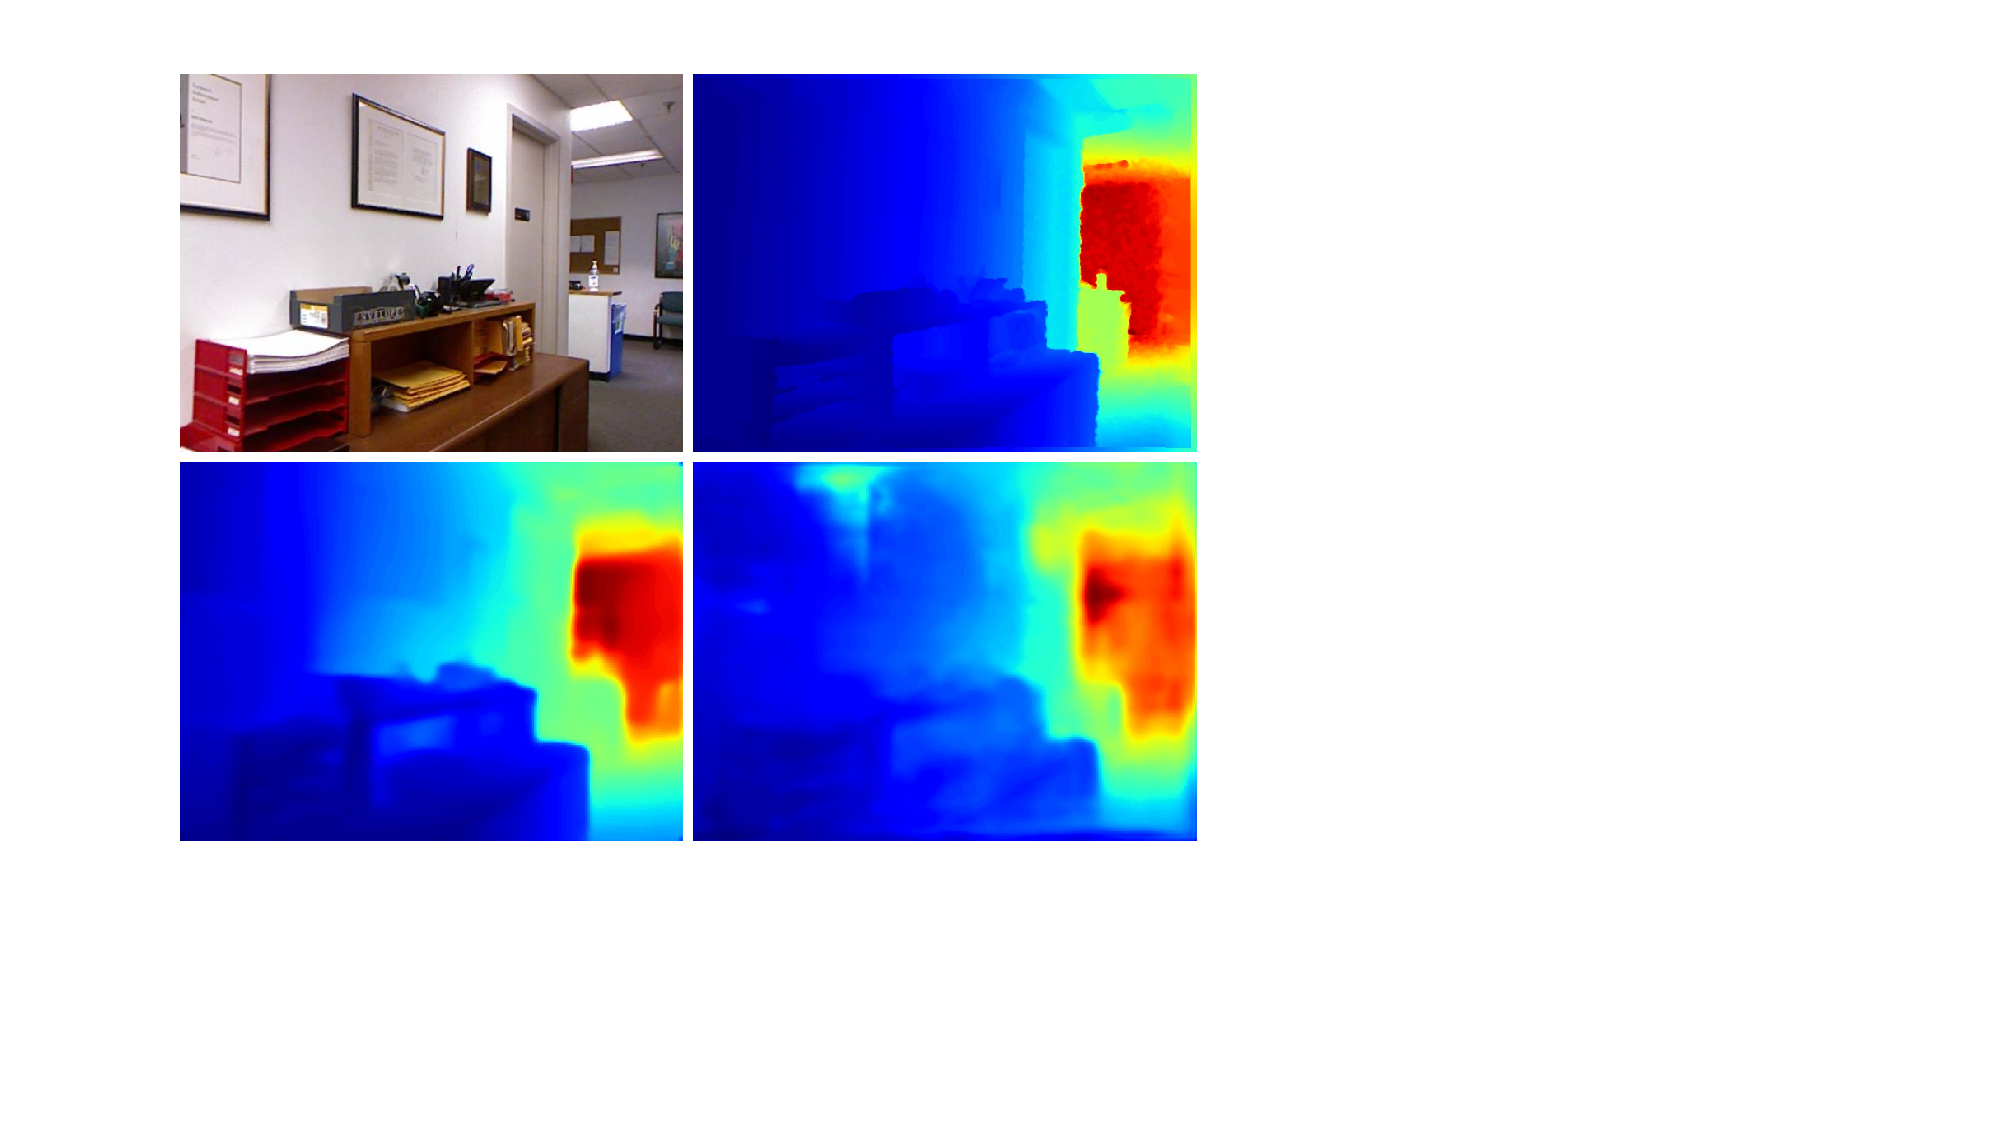
\includegraphics[width=0.95\linewidth]{figure/nyu_class_fail.pdf}
    \caption{}
    \end{subfigure}
    \begin{subfigure}{0.36\textwidth}
    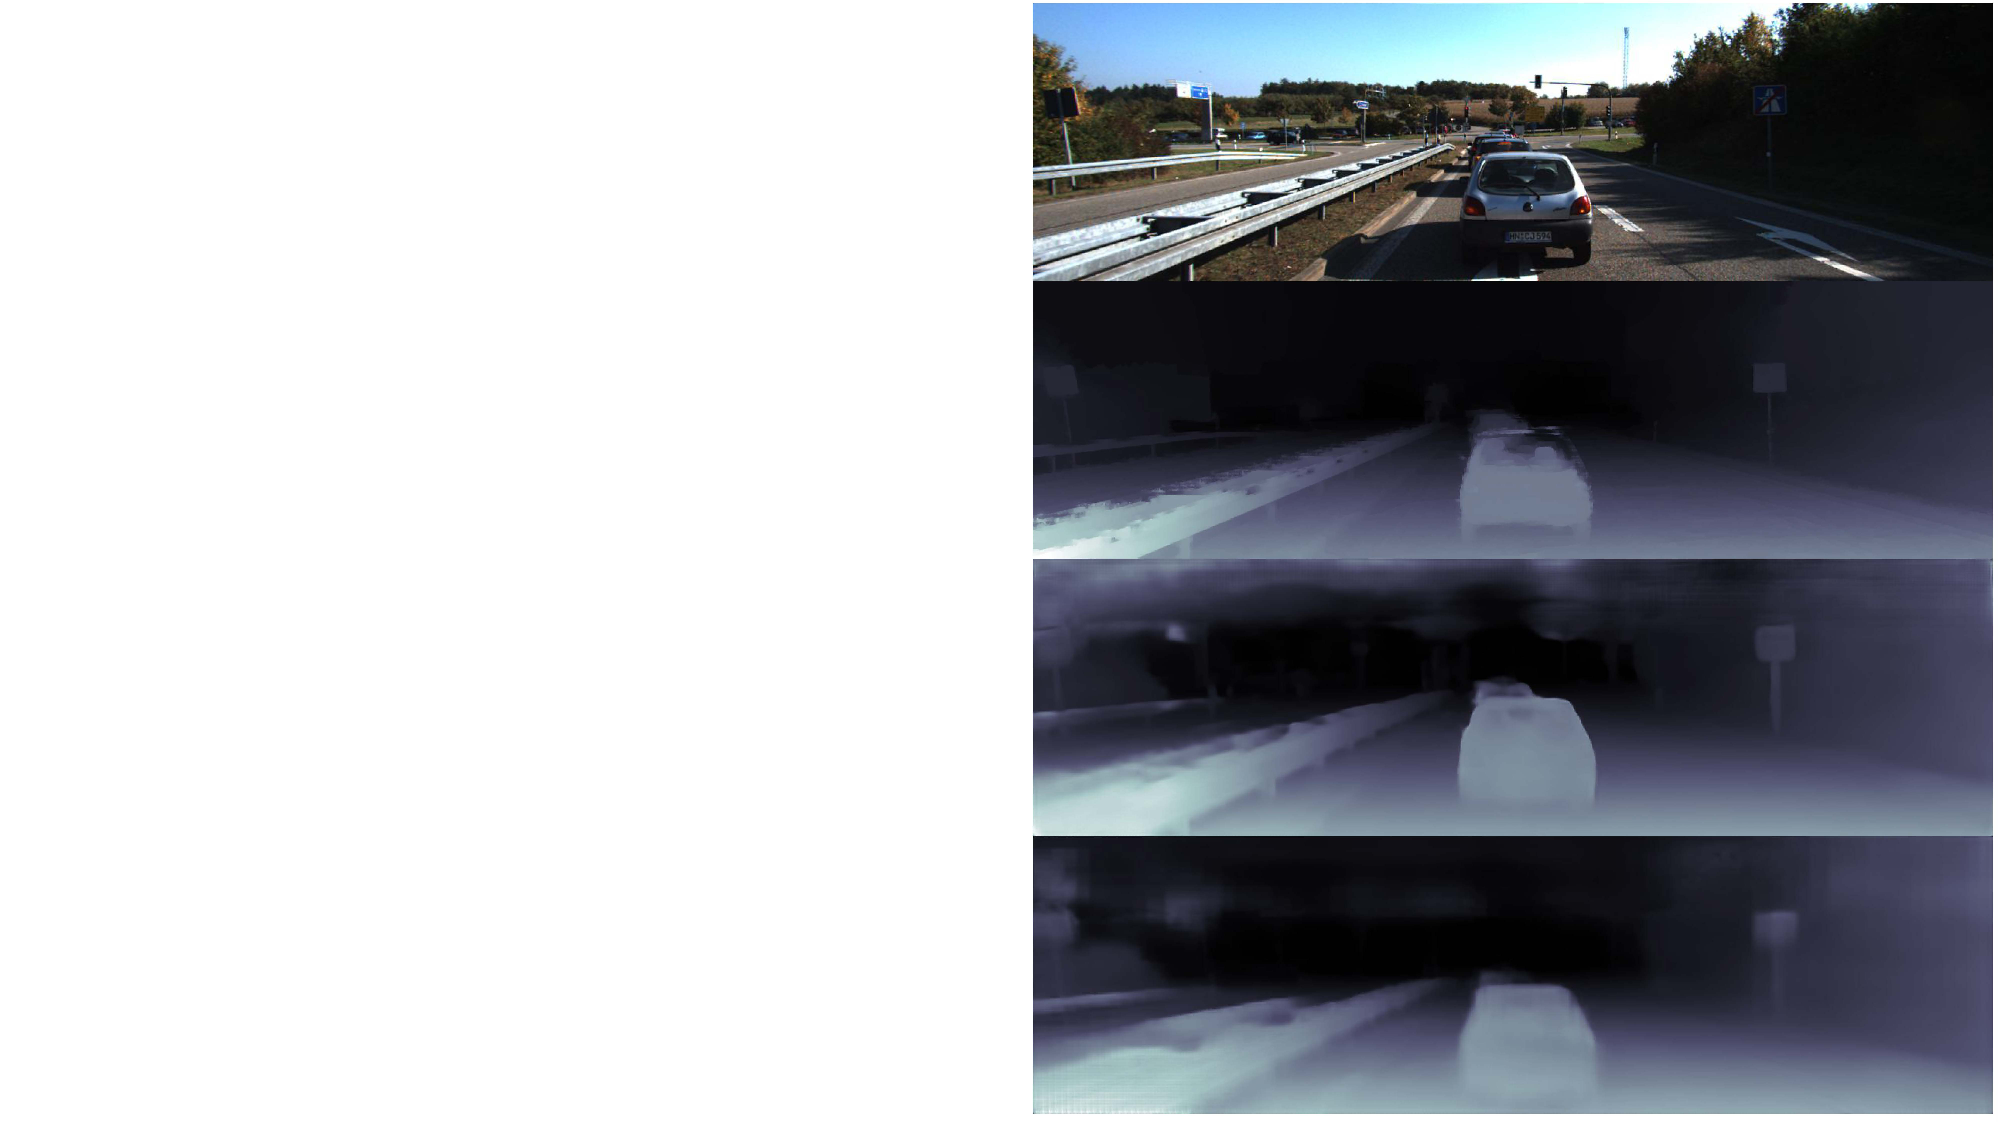
\includegraphics[width = 0.95\linewidth]{figure/kitti_bts_fail.pdf}
    \caption{}
    \end{subfigure}
    \caption{图(a)左上:RGB图像,右上:真实深度标注,左下:Li\cite{DABC}在NYU
    depth数据集上训练的预测图,右下:Li\cite{DABC}在联合数据集上训练的预测图。
    图(b)从上到下依次为:RGB图像,真实标注,BTS\cite{bts}在KITTI数据集
    上训练后的预测图,BTS\cite{bts}在联合数据集上训练的预测图。}
  \label{train_once_problem}
 \end{figure}
本章的创新点总结如下:
\begin{enumerate}
    \item 创新性地使用联合数据集
    来对网络进行训练测试,关注到了网络在对交叉场景的拟合和泛化能力。
    \item 提出了一种自蒸馏单目深度估计框架,一定程度上减弱了网络在面对复杂多样
    的数据分布时出现的性能退化现象,这种框架适用于所有的编解码网络,具有很强的移植性。
    \item 对比实验表明提出的框架对网络的拟合能力、泛化能力有了很大的提升。
\end{enumerate}

\section{自蒸馏单目深度估计框架}
\subsection{问题建模}
给定一个训练集 $\mathcal{T} = \{I,D\}$,
$I\in \mathcal{I}$, $D\in \mathcal{D}$,其中$\mathcal{I}$ 
和$\mathcal{D}$分别代表RGB图像集合和真实深度标注集合。
单目深度估计算法旨在得到RGB图像到深度图的映射:
$\varPhi:\mathcal{I}\rightarrow \mathcal{D}$。
当训练集包含复杂数据分布时
$\mathcal{T_{IO}} = \{(I_{in},I_{out}), (D_{in},D_{out})\}$,
其中$I/D_{in}$和$I/D_{out}$分别表示室内数据集和室外数据集。
算法需要强大的表达能力和拟合能力。

\begin{figure}[t]
    \centering
  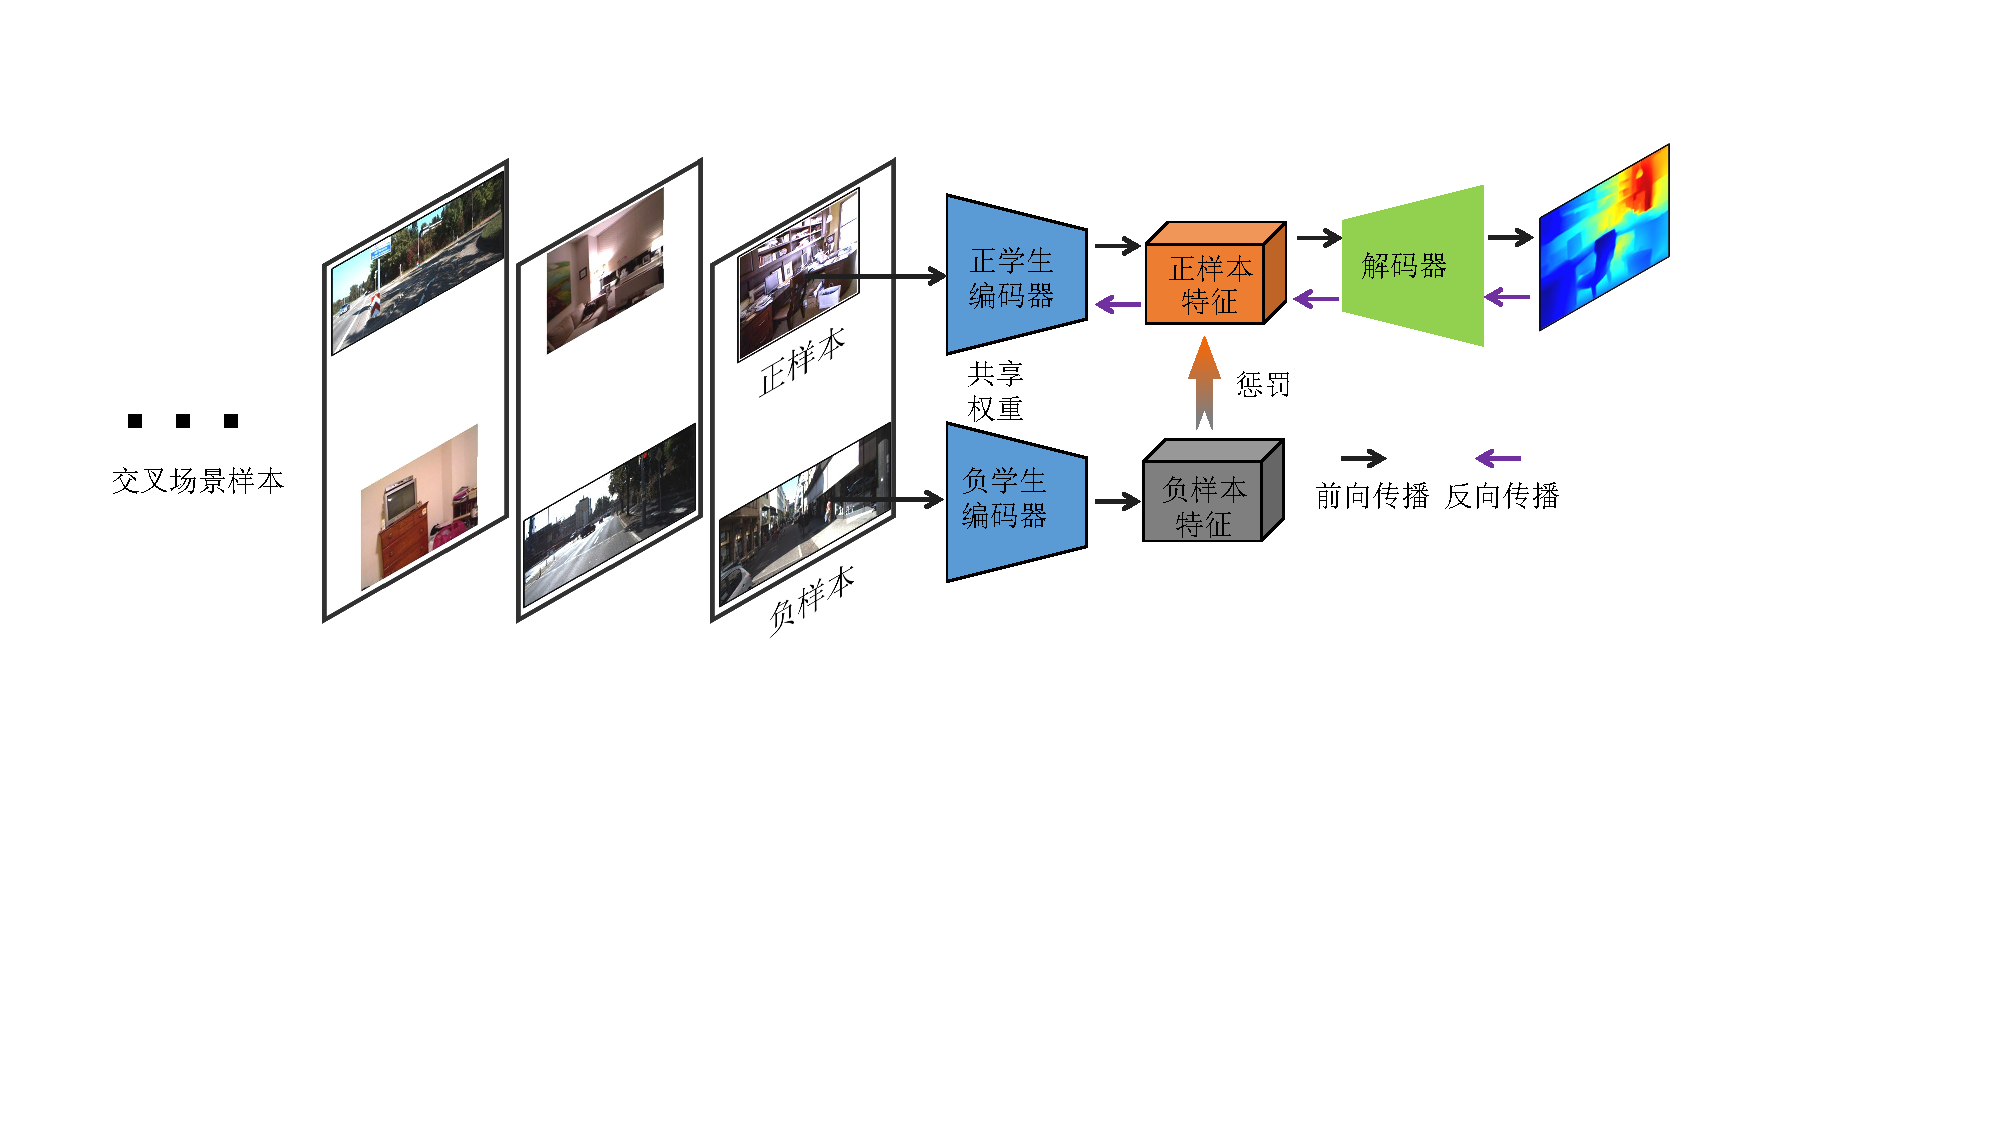
\includegraphics[width=1\linewidth]{figure/Stream.pdf}
  \centering
       \caption{针对复杂场景的自蒸馏深度估计框架}
   \label{Stream of algorithm} 
  \end{figure}
\subsection{网络结构}
\begin{algorithm*}[tbh]
  \caption{自蒸馏单目深度估计训练框架工作流程}
  \KwSty{需要训练的参数:}

      初始化KITTI参数:$\alpha$,
      NYU参数: $\beta$。
      
      \While{ $\alpha$ 或 $\beta$ 没有收敛} 
      {从KITTI或NYU数据集中随机采样一批图像

        \If(){采样了一批KITTI数据}{
          同时采样一批NYU数据\\
        \KwIn{将KITTI数据送入正学生编码器}
        通过优化损失函数$\mathcal{L}_{scale-invariant}$更新$\alpha$\\
        \KwIn{NYU数据被送入负学生编码器。}
        通过优化损失函数$\mathcal{L}_{dissimilarity}$来扩大
        $\beta$与$\alpha$之间的距离。
        }
        \If(){采样了一批NYU数据}{
          同时采样一批KITTI数据。\\
        \KwIn{将NYU数据送入正学生编码器}
        通过优化损失函数$\mathcal{L}_{scale-invariant}$更新$\beta$\\
        \KwIn{将KITTI数据被送入负学生编码器。}
        通过优化损失函数$\mathcal{L}_{dissimilarity}$来扩大
        $\alpha$与$\beta$之间的距离。
        }
      }
  \label{alg:backbone_alg}
  \end{algorithm*}
为了使算法可以更加鲁棒,首先构造了联合数据集(NYU depth和KITTI),
寄希望于算法在包含复杂场景的数据集下训练时,可以在复杂场景下
表现优异。但是随之而来的退化现象对网络的表达和拟合能力均是
一个挑战。
本章为了解决这种退化现象,采用了不同于以往的简单训练策略。
受到知识蒸馏网络的启发,设计了一种自蒸馏框架,
如图\ref{Stream of algorithm}所示。
框架同时从两个数据集分别进行采样,
正学生编码器提取正样本特征,同时负学生编码器提取另一数据集采样
的负样本的特征,负样本特征对正样本特征进行“惩罚”,
使$\mathbf{X_{IO}}$逐渐分化:
$\mathbf{X_{IO}} = \{\mathbf{X_{in}},\mathbf{X_{out}}\}$,
其中$\mathbf{X_{IO}}$代表包含室内特征和室外特征的复杂数据集。

本章采用目前最先进的算法之一BTS~\cite{bts}来实现编码器和解码器。
骨干网络采用了密集特征提取网络,得到了三个尺度
的特征图,它们的宽和高
分别为原尺寸1/2, 1/4, 1/8,随后最小的特征图经过了空洞空间金字塔模块
(Atrous Spatial Pyramid Pooling,ASPP),模块
空洞率分别为[3,6,12,18,24]。经过空洞空间金字塔池化模块
后,多尺度的语义信息被提取出来。随后每个尺度的特征图都
经过带有平面引导层
(Local Planar Guidance)的解码器,恢复为输入图原尺寸大小。
最后使用卷积层将不同尺度的预测图连接在一起计算出最终预测图。
本章设计了相异性损失函数Dissimilarity Loss使负样本对正样本进行“惩罚”,
从而使两个数据集的特征距离扩大。而该损失函数需要的特征向量需要
具有相同的尺寸,所以在编码器的最后一层,设计了
自适应池化层(Adaptive Pooling Layer)。
在经过自适应池化层之前,KITTI样本特征尺寸为$44\times88$,
而NYU depth样本特征尺寸为$52\times68$,
经过自适应池化层后他们的尺寸被统一调整为$44\times68$。
\begin{figure}[t]
    \centering
  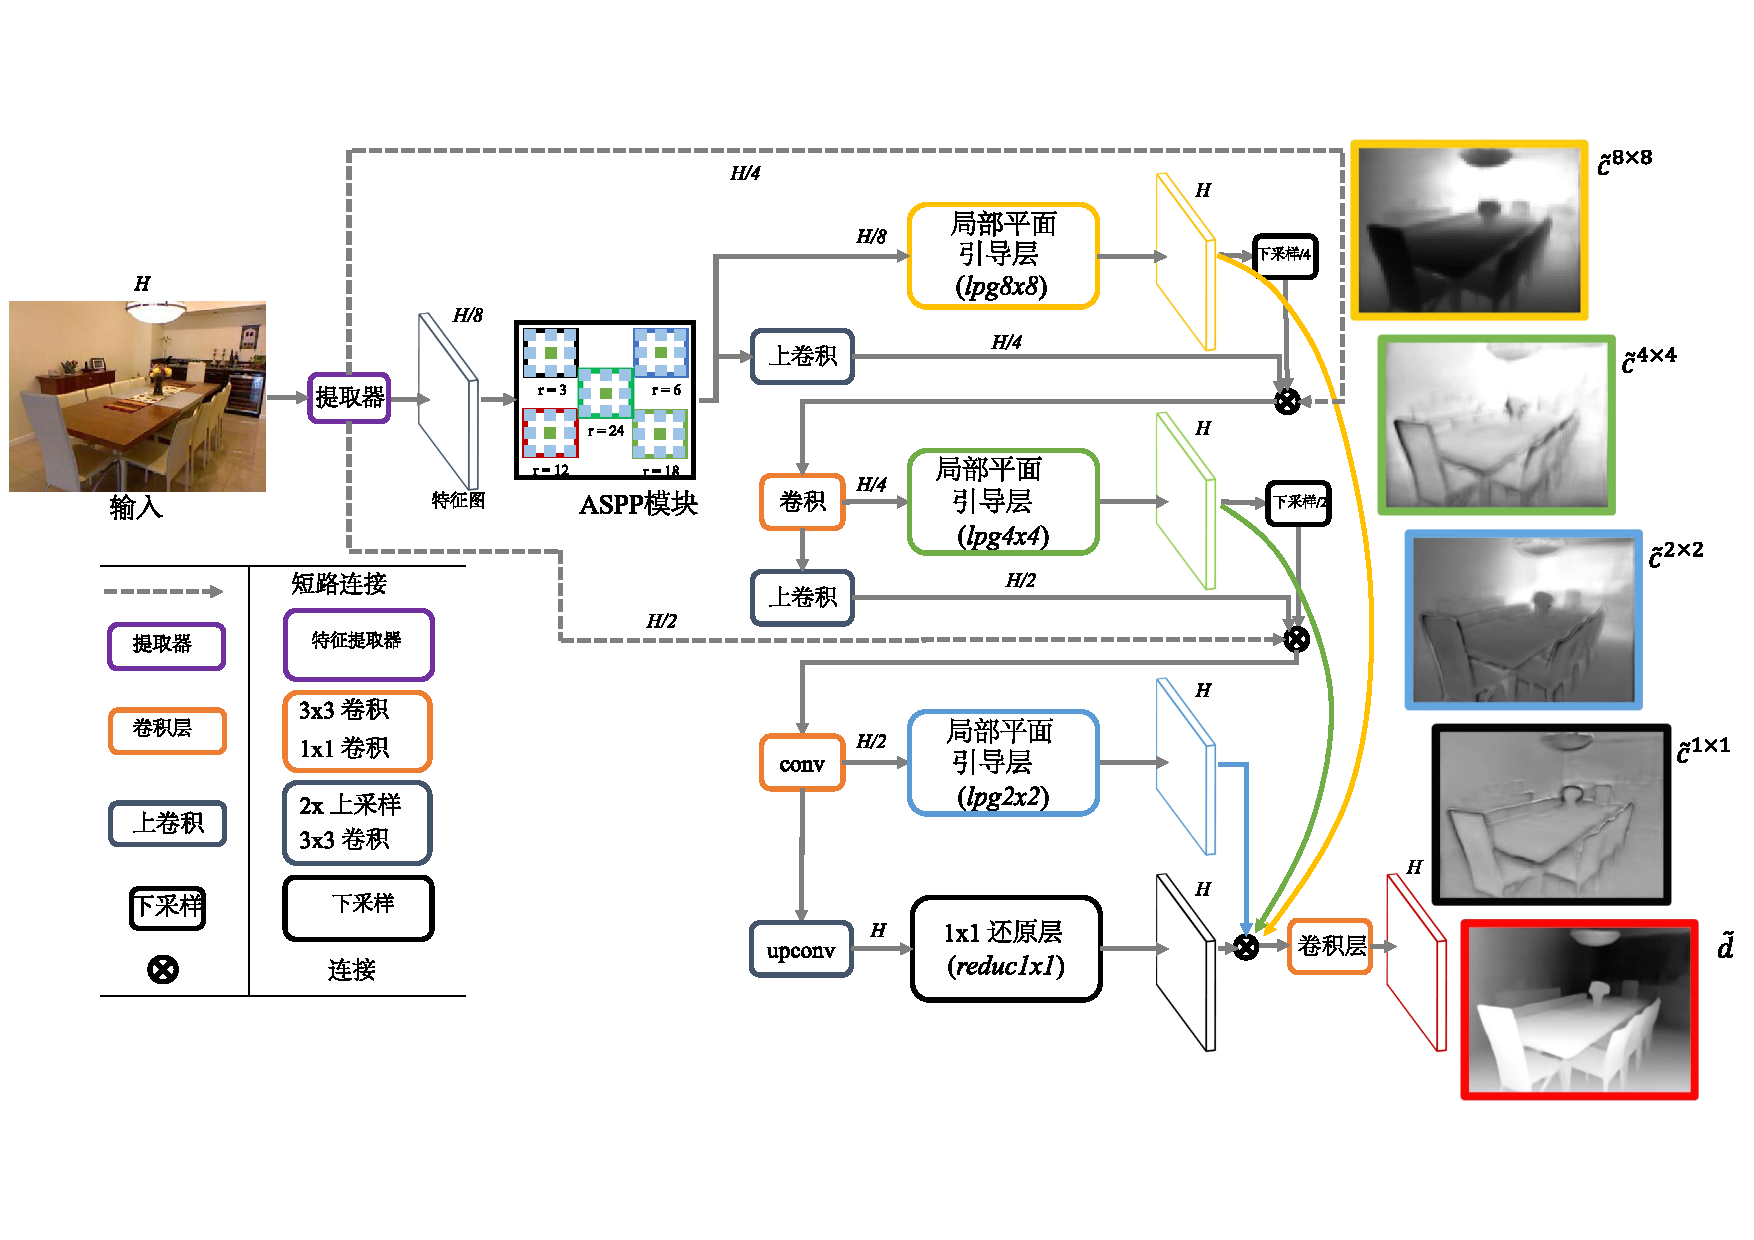
\includegraphics[width=1\linewidth]{figure/Bts_architecture.pdf}
  \centering
       \caption{自蒸馏框架使用的编解码器结构,采用了BTS\cite{bts}网络}
   \label{BTS architecture} 
  \end{figure}
 \subsection{损失函数}
一方面网络需要拟合两个数据集,另一方面网络又需要对两个
数据集进行区分,所以框架设计了两个损失函数,总的损失函数是两个
子损失函数项的线性加权。

学生编码器用来缩小相同数据集的类内间距,它由尺度一致性损失函数
\cite{eigen2014depth}来约束:
\begin{align}
  \mathcal{L}_{scale-invariant} = \frac{1}{N}\sum_{i}g_i^2-\frac{\lambda}{N^2}(\sum_{i}g_i)^2
\end{align}
其中$g_i=\log d_i^*-\log d_i$, $d_i^*$和$d_i$代表真实深度与
预测深度。$N$代表所有的像素数目。最后采用了BTS\cite{bts}
中的损失函数,因为BTS\cite{bts}证明了将损失函数的值域归一到一定范围
对预测效果有积极作用:
\begin{align}
 \mathcal{L}_{scale-invariant} = \alpha\sqrt{\frac{1}{N}\sum_{i}g_i^2-\frac{\lambda}{N^2}(\sum_{i}g_i)^2} 
\end{align}
$\alpha$在实验中被设置为10。

网络针对不同的彩色图产生相应的深度图,对网络的泛化性能
同样提出了要求。所以本章设计了$\mathcal{L}_
{dissimilarity}$来使网络对不同的数据集有所区分。
负学生编码器与正学生编码器共享权重,它
利用一组对应的样本,计算出负样本的
特征,这些特征通过dissmilarity loss的惩罚机制,不断扩大两个数据集
之间的类外间距: 
\begin{align}
  \mathcal{L}_{dissimilarity}=max(0,cos(\mathbf{x_f}, \mathbf{x_{nf}}) - margin)
\end{align} 
式中$margin$是一个系数并且在实验中设置为0。
$\mathbf{x_{f}}$和$\mathbf{x_{nf}}$分别代表正学生编码器与
负学生编码器计算的特征。
$cos(\mathbf{x_f}, \mathbf{x_{nf}})$代表两个特征图
的余弦相似性。实验中使用了$\mathbf{x_{f}}$ and $\mathbf{x_{nf}}$
沿通道维度的向量来计算余弦相似性。 

总的损失函数如下式所示:
\begin{align}
\mathcal{L} = \mathcal{L}_{scale-invariant} + \mathcal{L}_{dissimilary}
\end{align}
%(multiple means two here specially since we want our 
%subdatasets 
%contain same quality level images,so we discard
%Make3D~\cite{Make3D},
%which contains
%534 images and its images are too little to compare
%with KITTI~\cite{geiger2013vision} and NYU depth v2~\cite{Silberman:ECCV12}) at once with a semi-supervised way.

\section{实验结果与分析}
本节设计了几个实验来表明自蒸馏深度估计框架带来的提升。
包括与其他关键方法的直观衡量指标对比,与可视化结果对比。
除此之外,由于复杂数据集对单目深度估计网络的
表达能力和拟合能力都提出了新的要求,本节还通过
可视化卷积层的相关性来证明对表达能力和拟合能力的提升。
\subsection{实现细节}
\begin{figure*}[t]
  \centering
  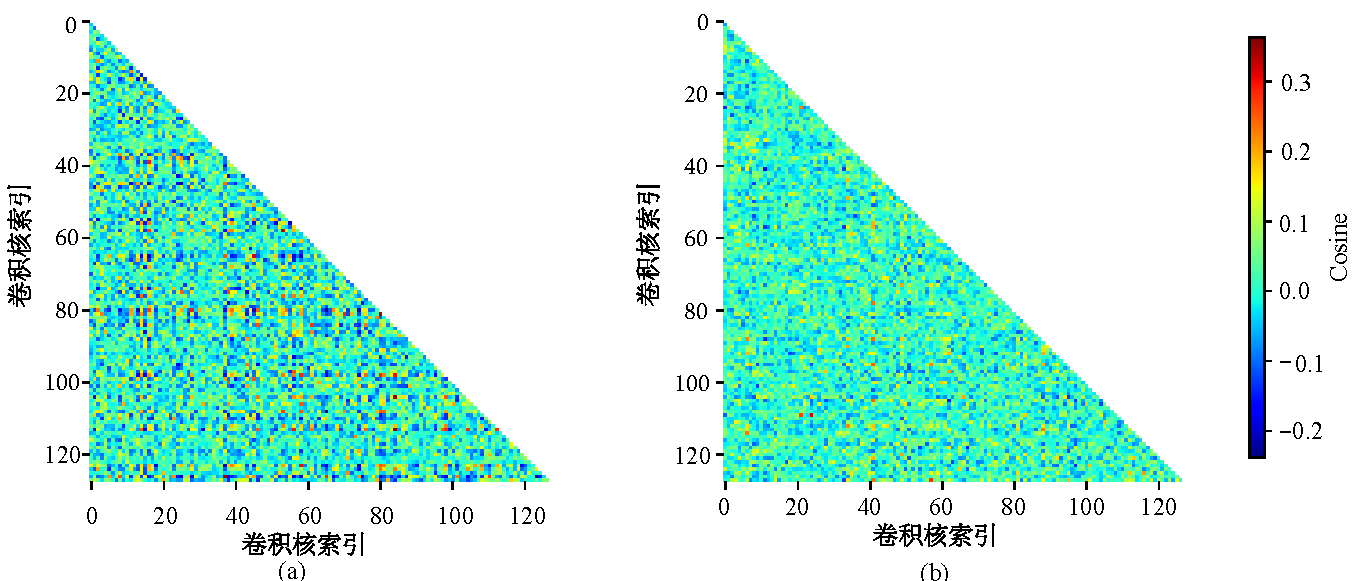
\includegraphics[width=0.85\linewidth]{figure/conv_co.pdf}
  \caption{编码器最后一层卷积核各通道之间的余弦相似性。
(a)为使用BTS~\cite{bts}采用常规训练框架时的卷积核通道相似性,
(b)为使用本章提出的自蒸馏框架训练的卷积核通道相似性。绿色代表
相似性越低。}
  \label{fig:conv_co}
  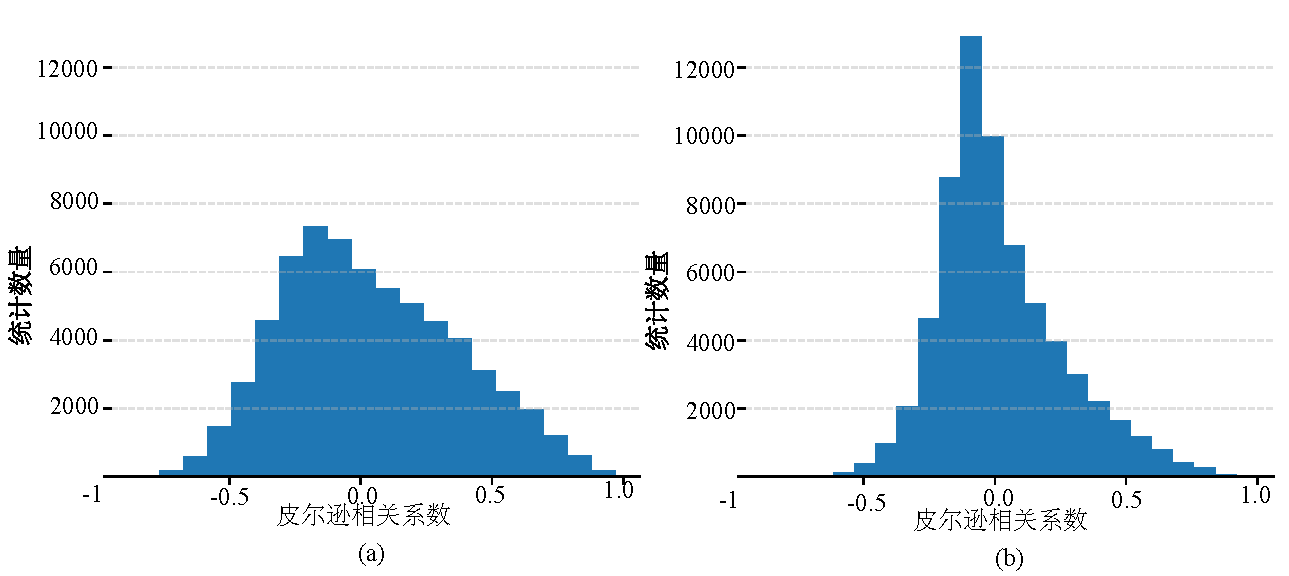
\includegraphics[width=0.85\linewidth]{figure/fea_co.pdf}
  \caption{特征图个通道间的皮尔逊相关系数的统计直方图,
  采用了[-1,-0.5],[-0.5,0],[0,0.5],[0.5,1]
  四个统计区间。(a)为使用常规训练框架训练得到的特征图的统计图,
  (b)为使用提出的自蒸馏框架训练得到的特征图的统计图。}
  \label{fig:fea_co}
\end{figure*}
本节所有实验的批尺寸均设置为4,并且设置了80000次迭代。因为KITTI
与NYU的图片同时被采样,也就是在同一批中,
但是两种数据的尺寸并不相同,其中NYU$416\times544$,KITTI
$352\times704$,所以需要将NYU图像进行左填充,将KITTI
图像进行右填充,是他们的尺寸同为$416\times704$,然后在送入网络之前,
在通过切片操作将其还原为各自尺寸。
数据增广方面,采用了与BTS~\cite{bts}相同的增广方法,
在对比度,光照,色彩调节方面,使用了范围在[0.9,1.1]
的随机调整。针对KITTI数据应用了[-2.5,2.5]的随机旋转操作,
针对NYU数据应用了[-1,1]的随机旋转操作。
整个实验实现使用了PyTorch~\cite{paszke2019pytorch}框架来完成。
\subsection{数据集与评价体系}
单目深度估计算法在室内场景和室外场景都应具有很强的鲁棒性。
然而,之前的工作一次只关注到一个场景,例如
在室外场景进行训练后测试,室内场景同理。
本章提出的算法旨在提升单目深度估计算法在室内外复杂场景
的鲁棒性,为了达到这个目的,本节在实验时组织了多个数据集,包括
室内数据集NYU depth和室外数据集KITTI。这两个数据集分别是
单目深度估计在室内场景和室外场景最常用的数据集。另外,
两个数据集包含的样本数量大致相当,相比之下Make3D和ScanNet
样本量太少,不适用于本章提出方法。

NYU depth v2数据集包含464个使用微软Kinect拍摄得室内场景
深度范围0到10m,根据Eigen\cite{eigen2014depth},实验中
从249个训练场景中选取了17000张图片以及其对应的深度图来构成
实验数据集。在测试部分仍然使用了官方发布的稠密标注测试集。
为了加速训练过程,对图像进行裁剪到$416 \times 544$。

KITTI数据集包含多个子任务数据集:物体检测,语义分割,深度估计,
深度补全等。这些子任务都是自动驾驶任务中的重点难点。深度信息和
彩色图像分别使用装载在行驶的车辆上的激光雷达与摄像机采集。
与现有工作一样,实验选取了22600张图像与对应点云组成复杂数据集。
点云在训练前使用补全方法进行了深度补全。KITTI图片被
裁剪为$352 \times 704$随后被送入网络。

为了客观公正的比较本章提出的框架,同时使方法对性能的提升有更直观的
体现,同样选取了五个广泛使用的指标\cite{eigen2014depth}:$
 RMSE=\sqrt{\frac{1}{\lvert N \rvert} \sum\nolimits_{i\in N}\lvert|d_i - d_i^*\rvert|^2} 
$,
$
  RMSE \ log = \sqrt{\frac{1}{\lvert N \rvert}\sum\nolimits_{i\in N}\lvert| \lg(d_i) - \lg(d_i^*) \rvert|^2}
$,
$
  Abs \ Rel=\frac{1}{\lvert N \rvert}\sum\nolimits_{i \in N}\frac{\lvert d_i - d_i^* \rvert}{d_i^*}
$,
$
  Sq \ Rel=\frac{1}{\lvert N \rvert}\sum\nolimits_{i \in N}\frac{\lvert| d_i - d_i^* \rvert|^2}{d_i^*}
$,
$
  Accuracies:\% \ of \ d_i \ s.t. \max(\frac{d_i}{d_i^*},\frac{d_i^*}{d_i})=\delta < thr 
$。
其中$d_i$和$d_i^*$表示预测深度与真实深度。$N$代表
所有的有效像素。 
\subsection{定量结果}

\begin{table*}[htb]
  \centering
  \caption{自蒸馏单目深度估计框架在NYU数据集的表现对比,最优结果使用加粗处理。}
  \label{tab:nyu quantitative result}
  \zihao{-5}
  \begin{tabular}{c|cc|cccc|ccc}
    \toprule
    \multirow{2}{*}{方法} & \multicolumn{2}{c|}{数据集}& \multicolumn{4}{c}{数值越低效果好}&\multicolumn{3}{|c}{数值越高效果越好}\\
    &KITTI&NYU& Rel Abs & Rel Sq & RMSE& RMSE $log$ &$\delta<1.25$ &$\delta<1.25^2$ & $\delta<1.25^3$ \\   
    \midrule
    Saxena\cite{Make3D}&&$\surd $&0.349&-&
    1.214&-&0.447&0.745&0.897\\
    Eigen\cite{eigen2014depth}&&$\surd$&0.215&-
    &0.907&0.282&0.702&0.898&0.967\\
    Liu\cite{liu2015learning}&&$\surd$&0.213&-&0.759&-&0.650&0.906&0.976\\
    Chakrabarti\cite{chakrabarti2016depth}&&$\surd$&0.149&-&0.620&-&0.806&0.953&0.988\\
    Laina\cite{laina2016deeper}&&$\surd$&0.114&0.898&4.935&0.206&0.861&0.949&0.976\\
    Lee\cite{lee2019monocular}&&$\surd$&
    0.131&0.087&0.538&-&0.837&0.971&0.994\\
    Fu\cite{FuCVPR18-DORN}&&$\surd$&0.115&-&0.509&-&0.828&0.965&0.992\\
    Xu\cite{xu2018structured}&&$\surd$&0.125&-&0.593&-&0.806&0.952&0.986\\
    \hline
    Li\cite{DABC}&&$\surd$&0.124&&0.597&0.366&0.814&0.960&0.988\\
    Li\cite{DABC}&$\surd$&$\surd$&0.174&-&0.796&0.401&0.724&0.911&0.942\\
    \hline
    BTS\cite{bts}&&$\surd$&\textbf{0.110}&-&0.392&\textbf{0.047}&\textbf{0.885}&\textbf{0.978}&\textbf{0.994}\\
    BTS\cite{bts}&$\surd$&$\surd$&0.172&0.101&0.402&0.198&0.731&0.933&0.984\\
    Ours&$\surd$&$\surd$&0.163&\textbf{0.091}&\textbf{0.388}&0.190&0.746&0.941&0.987\\
    \bottomrule
  \end{tabular}
\end{table*}
本节使用Eigen\cite{eigen2014depth}在KITTI与NYU测试数据集上
测试了提出的框架。注意实验使用组合复杂数据集进行训练,随后使用
各自的测试集对网络进行测试。在表
\ref{tab:nyu quantitative result}中使用领域关键方法
作为基准,包括
Eigen\cite{eigen2014depth},Liu\cite{liu2015learning}, 
Chakrabarti\cite{chakrabarti2016depth}, 
Laina\cite{laina2016deeper}, Lee\cite{lee2019monocular}等方法。
通过对比发现,当使用复合数据集进行训练时,Li\cite{DABC}与
BTS\cite{bts}均有不同程度的退化现象。在Rel Abs指标上
分别有40\%和56\%的衰退。单数据集表现上,BTS\cite{bts}
在大多数指标上都取得了最优的结果。当使用复杂数据集时,应用了
自蒸馏深度估计框架可以使所有指标均获得一定的提升,其中
Rel Sq, RMSE指标分别获得10\%和3\%的提升后甚至超越了在单数据集
上的表现,达到了最优效果。在正确估计像素的占比上,该框架同样
可以减缓面对复杂数据集的衰退现象。


\begin{table*}[htb]
  \centering
  \caption{自蒸馏单目深度估计框架在KITTI数据集表现对比,最优结果使用加粗处理。}
  \label{tab:kitti quantitative result}
  \zihao{-5}
  \begin{tabular}{c|cc|cccc|ccc}
    \toprule
    \multirow{2}{*}{方法} & \multicolumn{2}{c|}{数据集}& \multicolumn{4}{c|}{数值越低效果越好}&\multicolumn{3}{c}{数值越高效果越好}\\
    &KITTI&NYU& Rel Abs & Rel Sq & RMSE& RMSE $log$ &$\delta<1.25$ &$\delta<1.25^2$ & $\delta<1.25^3$ \\   
    \midrule
    Saxena\cite{Make3D}&$\surd $&&0.280&3.012&
    8.734&0.361&0.601&0.820&0.926\\
    Eigen\cite{eigen2014depth}&$\surd$&&0.203&
    1.548&6.307&0.282&0.702&0.898&0.967\\
    Liu\cite{liu2015learning}&$\surd$&&0.201&1.584&6.471&0.273&0.680&0.898&0.967\\
    Kuznietsov\cite{kuznietsov}&$\surd$&&0.113&0.741&4.621&0.189&0.862&0.960&0.986\\

    Godard\cite{godard2017unsupervised}&$\surd$&&0.114&0.898&4.935&0.206&0.861&0.949&0.976\\
    Zhow\cite{zhou2017unsupervised}&$\surd$&&
    0.198&1.836&6.565&0.275&0.718&0.901&0.960\\
    Fu\cite{FuCVPR18-DORN}&$\surd$&&0.072&0.307&\textbf{2.727}&0.120&0.932&0.984&0.994\\
    Xu\cite{xu2018structured}&$\surd$&&0.122&0.897&4.677&-&0.818&0.954&0.850\\
    \hline
    Li\cite{DABC}&$\surd$&&0.144&0.528&4.470&0.197&0.845&0.961&0.984\\
    Li\cite{DABC}&$\surd$&$\surd$&0.231&0.655&7.096&0.259&0.734&0.891&0.921\\
    \hline
    BTS\cite{bts}&$\surd$&&\textbf{0.059}&\textbf{0.245}&2.756&\textbf{0.096}&\textbf{0.956}&\textbf{0.993}&\textbf{0.998}\\
    BTS\cite{bts}&$\surd$&$\surd$&0.114&0.392&3.257&0.142&0.892&0.989&\textbf{0.998}\\
    Ours&$\surd$&$\surd$&0.115&0.389&3.036&0.144&0.890&0.989&\textbf{0.998}\\
    \bottomrule
  \end{tabular}
\end{table*}
表\ref{tab:kitti quantitative result}展示了框架在KITTI数据集
上的表现。实验同样选取了Li\cite{DABC}与BTS\cite{bts}作为
对比基准。两种方法的各个指标当使用复杂数据集时也出现了不同程度的衰退。
这再一次证明了常规方法在面对复杂数据分布时的不足。
Fu\cite{FuCVPR18-DORN}在RMSE指标上取得了最优的效果,
但是在其他指标上,BTS\cite{bts}取得了最优的结果。本章提出的框架
未能使任何指标反超BTS\cite{bts}在面对单一KITTI时的表现,但是在
$\delta<1.25^3$指标上与单一数据集的表现达到了持平。

\subsection{视觉效果}

面对特定的场景,鲁棒的单目深度估计算法可以生成特定精准的深度图,
本章方法针对不同的场景可以提取不同的特征图。
但是网络的表达能力同样扮演了重要的角色,因为
网络需要从提取的密度特征来生成最终的深度图。
本节计算了自适应池化层之前的卷积层各通道之间的
余弦相似性。图\ref{fig:conv_co}表明本框架可以降低网络卷积通道之间
的相关性,从而降低卷积核的冗余性。但是图(a)表明,在复杂数据集上的
常规训练方式使得网络仍然具有很强的冗余性,进而降低了网络的表达能力。
实验还计算了编码器产生的特征图通道之间的皮尔逊相关系数
(Pearson Correlation Coefficient, PCC)。
具体计算方式如下:特征图具有128个通道,将特征图的
长、宽维度展开,使其尺寸变为$128\times\mathbf{(H\times W)}$,
随后计算了特征图每个通道之间的皮尔逊相关系数,如图
\ref{fig:fea_co}所示。 与简单的使用复杂数据集训练相比,
本章自蒸馏框架产生的特征图通道之间的皮尔逊相关系数更多的集中在0
附近,即具有更少的相关性。但是图(a)中展示的统计图,
通道之间的相关性较为分散,具有较强的相关性,即特征图
并没有被很好的分化。

\begin{figure*}[htb]
  \centering
  \begin{subfigure}{0.15\linewidth}
  \begin{minipage}[b]{1\linewidth}
  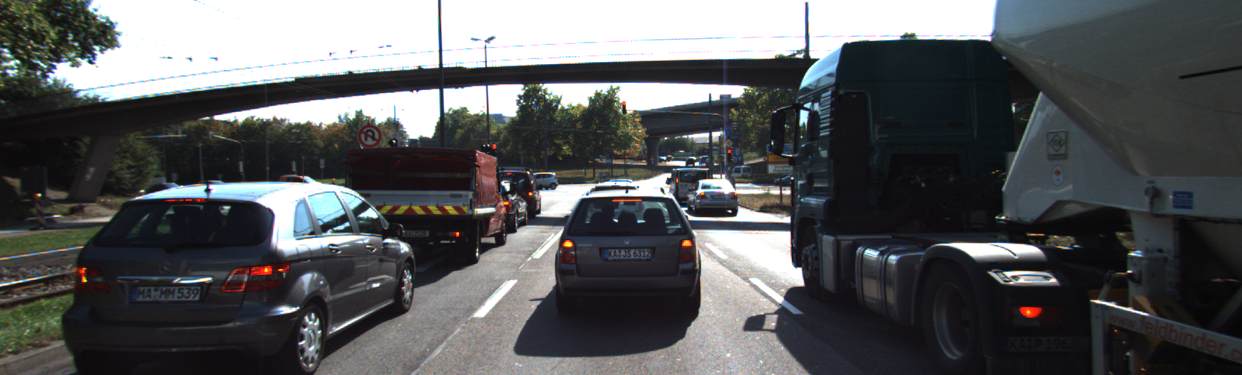
\includegraphics[width=1\linewidth]{figure/kitti_rgb/0000000000.png}\vspace{4pt}
  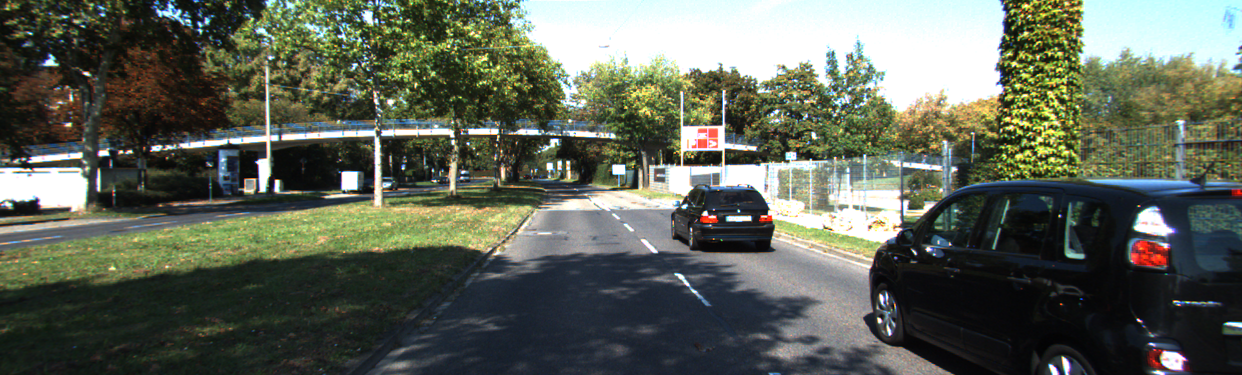
\includegraphics[width=1\linewidth]{figure/kitti_rgb/0000000035.png}\vspace{4pt}
  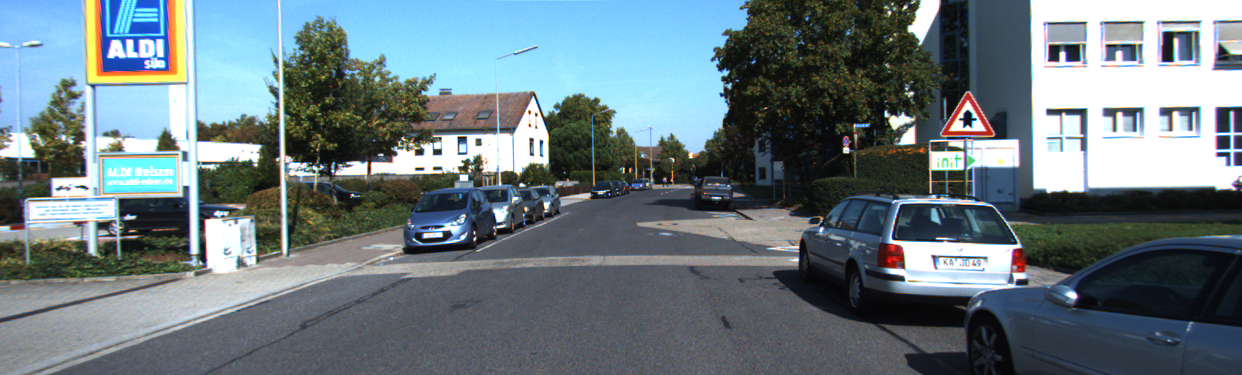
\includegraphics[width=1\linewidth]{figure/kitti_rgb/0000000260.png}\vspace{4pt}
  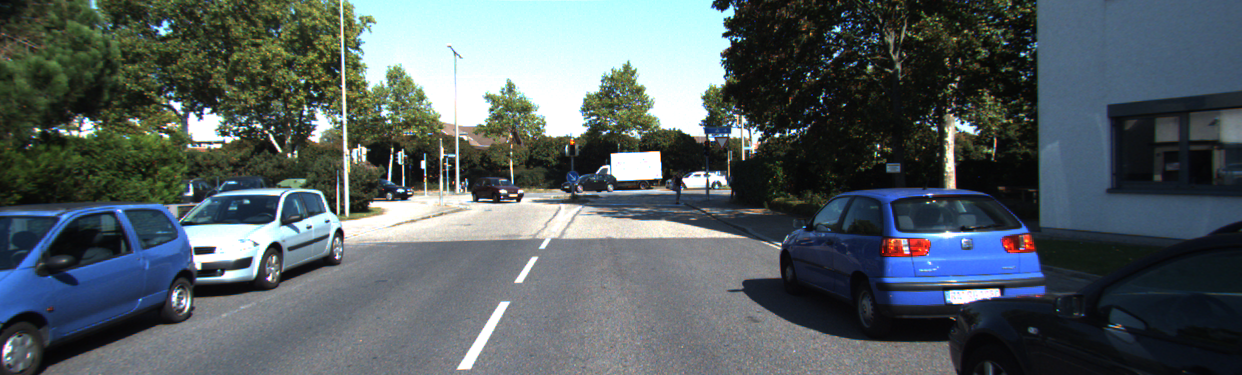
\includegraphics[width=1\linewidth]{figure/kitti_rgb/0000000340.png}\vspace{4pt}
  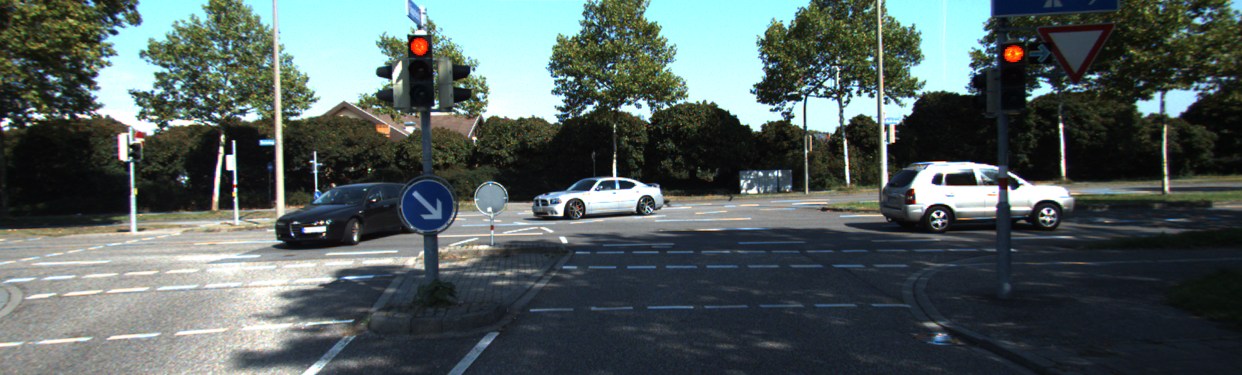
\includegraphics[width=1\linewidth]{figure/kitti_rgb/0000000388.png}\vspace{4pt}
  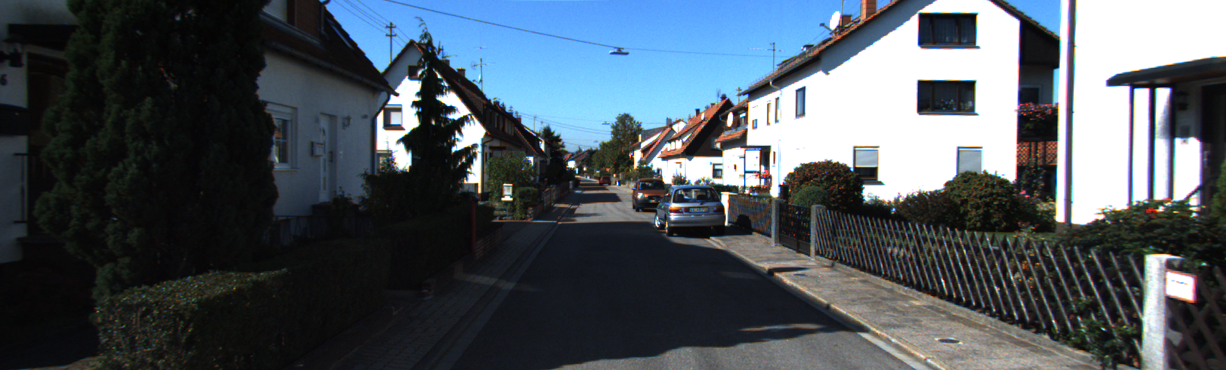
\includegraphics[width=1\linewidth]{figure/kitti_rgb/0000000642.png}
  \end{minipage}
  \caption{RGB图像}
  \end{subfigure}
  \begin{subfigure}{0.15\linewidth}
  \begin{minipage}[b]{1\linewidth}
  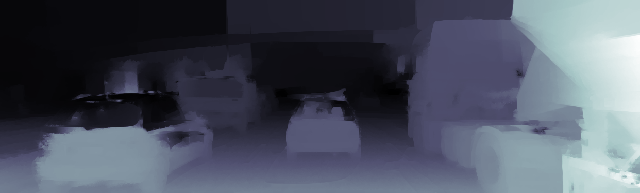
\includegraphics[width=1\linewidth]{figure/kitti_gt/26_52_00.png}\vspace{4pt}
  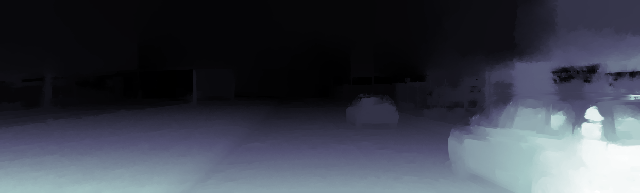
\includegraphics[width=1\linewidth]{figure/kitti_gt/26_13_35.png}\vspace{4pt}
  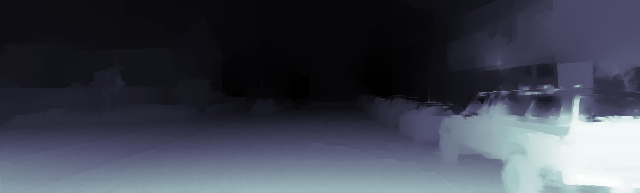
\includegraphics[width=1\linewidth]{figure/kitti_gt/26_09_260.png}\vspace{4pt}
  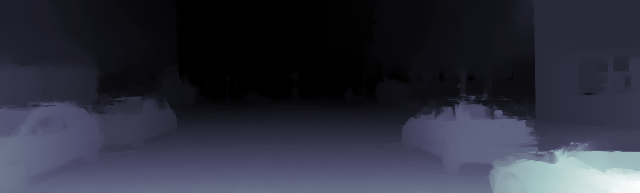
\includegraphics[width=1\linewidth]{figure/kitti_gt/26_09_340.png}\vspace{4pt}
  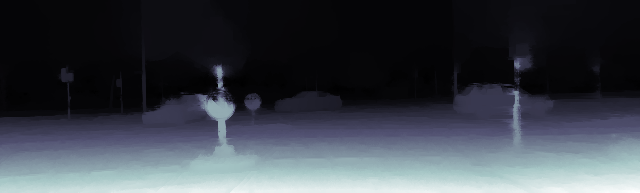
\includegraphics[width=1\linewidth]{figure/kitti_gt/26_09_388.png}\vspace{4pt}
  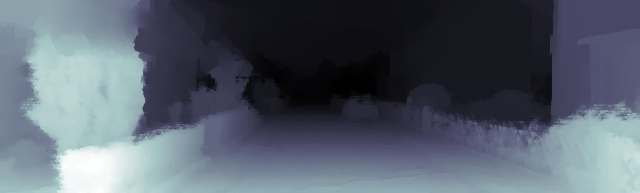
\includegraphics[width=1\linewidth]{figure/kitti_gt/30_18_642.png}
  \end{minipage}
  \caption{真实标注}
  \end{subfigure}
  \begin{subfigure}{0.15\linewidth}
  \begin{minipage}[b]{1\linewidth}
  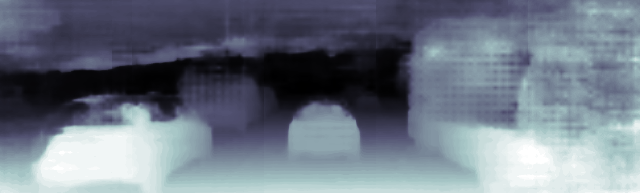
\includegraphics[width=1\linewidth]{figure/dorn/2011_09_26_drive_0052_sync_0000000000.png}\vspace{4pt}
  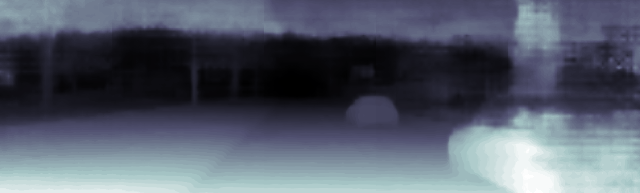
\includegraphics[width=1\linewidth]{figure/dorn/2011_09_26_drive_0013_sync_0000000035.png}\vspace{4pt}
  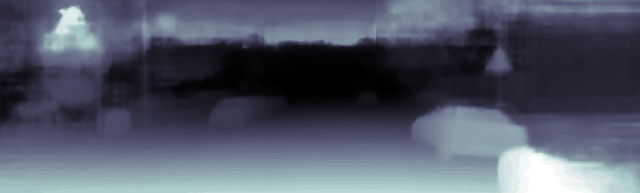
\includegraphics[width=1\linewidth]{figure/dorn/2011_09_26_drive_0009_sync_0000000260.png}\vspace{4pt}
  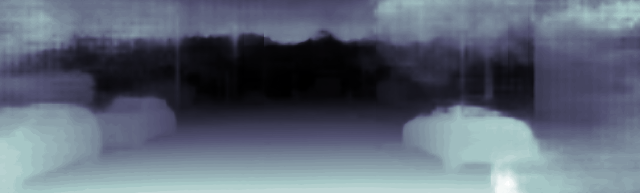
\includegraphics[width=1\linewidth]{figure/dorn/2011_09_26_drive_0009_sync_0000000340.png}\vspace{4pt}
  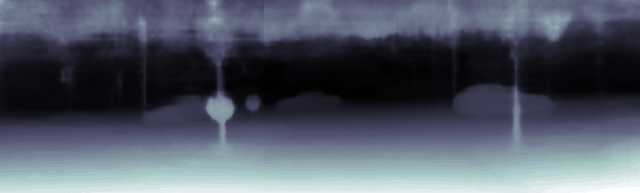
\includegraphics[width=1\linewidth]{figure/dorn/2011_09_26_drive_0009_sync_0000000388.png}\vspace{4pt}
  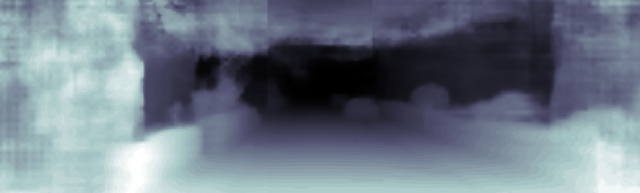
\includegraphics[width=1\linewidth]{figure/dorn/2011_09_30_drive_0018_sync_0000000642.png}
  \end{minipage}
  \caption{DORN~\cite{FuCVPR18-DORN}}
  \end{subfigure}
  \begin{subfigure}{0.15\linewidth}
  \begin{minipage}[b]{1\linewidth}
  
\includegraphics[width=1\linewidth]{figure/kitti_sfm/2011_09_26_drive_0052_sync_0000000000.png}\vspace{3.5pt}
  
\includegraphics[width=1\linewidth]{figure/kitti_sfm/2011_09_26_drive_0013_sync_0000000035.png}\vspace{3.5pt}
  
\includegraphics[width=1\linewidth]{figure/kitti_sfm/2011_09_26_drive_0009_sync_0000000260.png}\vspace{3.5pt}
  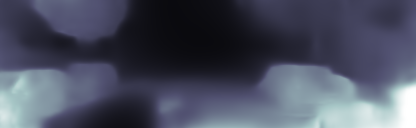
\includegraphics[width=1\linewidth]{figure/kitti_sfm/2011_09_26_drive_0009_sync_0000000340.png}\vspace{3.5pt}
  
\includegraphics[width=1\linewidth]{figure/kitti_sfm/2011_09_26_drive_0009_sync_0000000388.png}\vspace{3.5pt}
  
\includegraphics[width=1\linewidth]{figure/kitti_sfm/2011_09_30_drive_0018_sync_0000000642.png}
  \end{minipage}
  \caption{SfmLearner~\cite{zhou2017unsupervised}}
  \end{subfigure}
  \begin{subfigure}{0.15\linewidth}
  \begin{minipage}[b]{1\linewidth}
  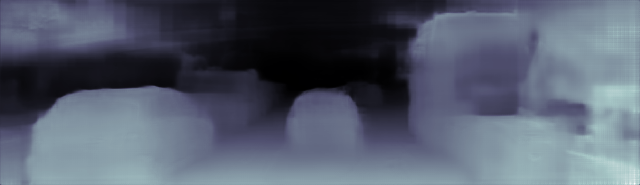
\includegraphics[width=1\linewidth]{figure/kitti_without/2011_09_26_drive_0052_sync_0000000000.png}\vspace{5pt}
  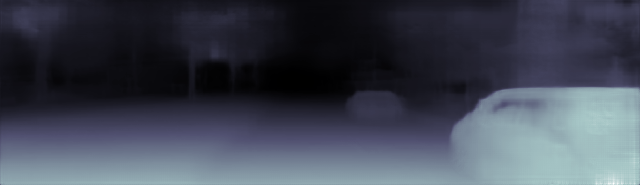
\includegraphics[width=1\linewidth]{figure/kitti_without/2011_09_26_drive_0013_sync_0000000035.png}\vspace{5pt}
  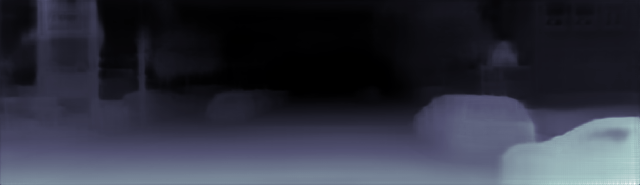
\includegraphics[width=1\linewidth]{figure/kitti_without/2011_09_26_drive_0009_sync_0000000260.png}\vspace{5pt}
  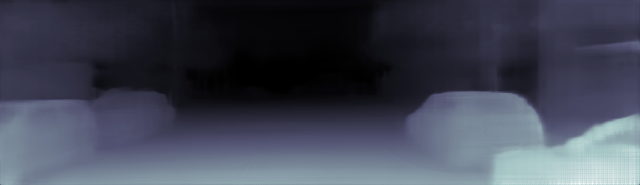
\includegraphics[width=1\linewidth]{figure/kitti_without/2011_09_26_drive_0009_sync_0000000340.png}\vspace{5pt}
  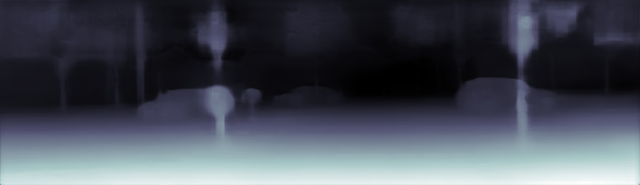
\includegraphics[width=1\linewidth]{figure/kitti_without/2011_09_26_drive_0009_sync_0000000388.png}\vspace{5pt}
  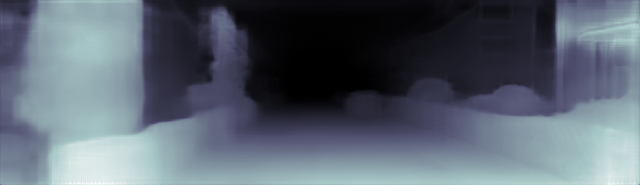
\includegraphics[width=1\linewidth]{figure/kitti_without/2011_09_30_drive_0018_sync_0000000642.png}
  \end{minipage}
  \caption{BTS\cite{bts}}
  \end{subfigure}
  \begin{subfigure}{0.15\linewidth}
  \begin{minipage}[b]{1\linewidth}
  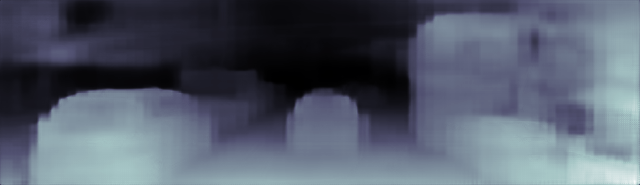
\includegraphics[width=1\linewidth]{figure/kitti_result/2011_09_26_drive_0052_sync_0000000000.png}\vspace{5pt}
  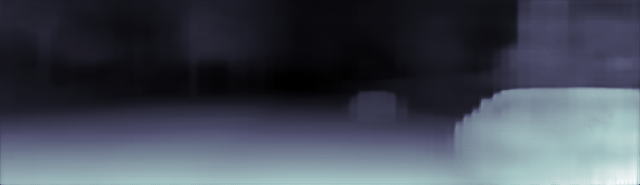
\includegraphics[width=1\linewidth]{figure/kitti_result/2011_09_26_drive_0013_sync_0000000035.png}\vspace{5pt}
  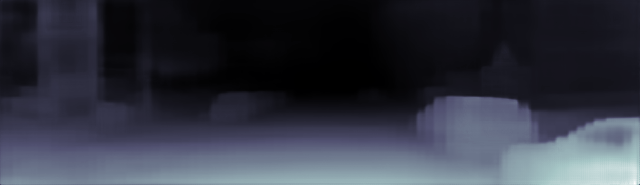
\includegraphics[width=1\linewidth]{figure/kitti_result/2011_09_26_drive_0009_sync_0000000260.png}\vspace{5pt}
  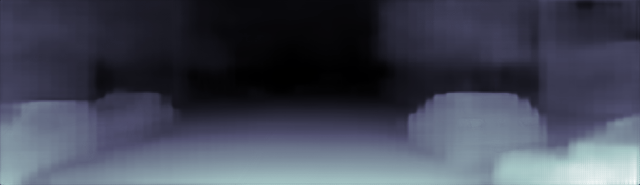
\includegraphics[width=1\linewidth]{figure/kitti_result/2011_09_26_drive_0009_sync_0000000340.png}\vspace{5pt}
  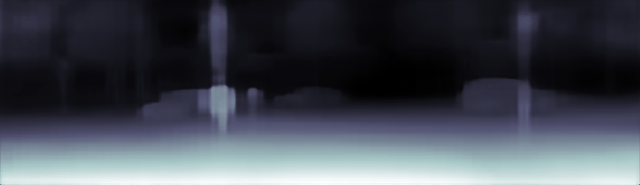
\includegraphics[width=1\linewidth]{figure/kitti_result/2011_09_26_drive_0009_sync_0000000388.png}\vspace{5pt}
  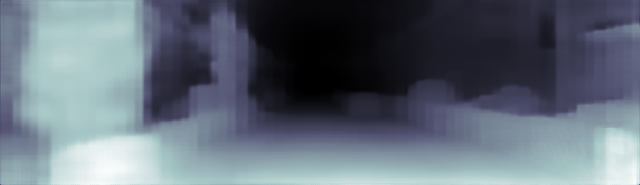
\includegraphics[width=1\linewidth]{figure/kitti_result/2011_09_30_drive_0018_sync_0000000642.png}
  \end{minipage}
  \caption{Ours}
  \end{subfigure}
  \begin{subfigure}{1\linewidth}
    \begin{minipage}[]{0.5\linewidth}
    \centering
     \includegraphics[width=0.95\linewidth]{figure/without_error.png} 
    \end{minipage}
    \begin{minipage}[]{0.5\linewidth}
    \centering
     \includegraphics[width=0.95\linewidth]{figure/our_error.png} 
    \end{minipage}
  \end{subfigure}
  \caption{预测结果的可视化对比,对比图中的稀疏真实深度点云使用了
  NYU depth提供的工具箱进行了填充。
  请注意DORN\cite{FuCVPR18-DORN}与SfmLearner\cite{zhou2017unsupervised}
  仅仅使用了KITTI数据集进行了训练,BTS\cite{bts}与本章所用方法
  均使用了复合数据集。热力图为最后一张图像的预测误差图,
  ($map_{error} = D_{gt} - D_{pre}$),左图为BTS\cite{bts}预测误差图,
  右图为本章框架的预测误差图。}
  \label{KITTI visualization result}
  \end{figure*}

实验同样进行了可视化对比。本节展示了与领先方法的视觉效果对比,
如图\ref{KITTI visualization result}所示。相比
DORN\cite{FuCVPR18-DORN}与SfmLearner\cite{zhou2017unsupervised}
本章方法在边界重建和深度精度上都表现良好。
DORN\cite{FuCVPR18-DORN}方法在天空部分预测出现了较大的误差,
而SfmLearner\cite{zhou2017unsupervised}预测的深度图
物体轮廓不够明显。相比BTS\cite{bts},使用本框架时出现了一些锯齿化现象,
这可能是由于添加了自适应池化层造成的。为了更好地展示
框架带来的效果提升,图\ref{KITTI visualization result}
最后一行展示了放大的预测误差图。图左为最后一张RGB图像
使用BTS在复杂数据集训练后预测深度图的误差图,图右为
使用自蒸馏框架在复杂数据集训练后预测深度图的误差图,可以
本章提出的自蒸馏框架对效果有着明显的提升。可以发现自蒸馏框架的加入
使得网络在远距离的预测误差(蓝色区域)大幅减少。

NYU数据集上的视觉对比如图\ref{nyu visualization result}所示,
自蒸馏框架在细节的预测上表现优异,如第一幅图像中的书架,
第四幅图中的人像,
第五幅图像中的浴缸等。

\subsection{算法复杂度分析}
本节重点分析该自蒸馏框架的时间与空间复杂度,以
验证该系统后续在线使用的可能性。由于框架适用于大多数
编解码网络,所以框架实际复杂度与所采用的编解码结构有关,
本节分析
了使用BTS\cite{bts}作为编解码结构的自蒸馏框架复杂度。本实验
采用了四张英伟达2080TI显卡,
Intel(R) Xeon(R) CPU E5-2678 v3 @ 2.50GHz cpu
来搭建硬件实验平台。软件方面,使用了英伟达418.56
版本驱动,CUDA使用了10.1版本,pytorch使用了1.1.0版本来进行
算法实现。
在训练时间上,该框架经过了学生编码器和负学生编码器的两次前项推理和
一次反向传播过程,完成一个训练周期,共计46672张图像训练
耗时3.12h,平均每张图片耗时0.24s。在推理阶段,
平均每张图片耗时0.09s。每次迭代自蒸馏框架浮点运算量
为1.18TFLOPs。在空间复杂度上,自蒸馏框架共计73848300个参数
其中可训练参数为73790040个,但是由于自蒸馏框架在推理阶段不需要
负学生编码器,所以只有47000688个参数。

\begin{figure*}[htb]
  \centering
  \begin{subfigure}{0.15\linewidth}
    
  \begin{minipage}[t]{1\linewidth}
  \centering
  \includegraphics[width=1\linewidth]{figure/nyu_rgb/15.png}
  \includegraphics[width=1\linewidth]{figure/nyu_gt/15.png}
  \includegraphics[width=1\linewidth]{figure/nyu_result/office_rgb_00015.png}
  \includegraphics[width=1\linewidth]{figure/nyu_without/office_rgb_00015.png}
  \includegraphics[width=1\linewidth]{figure/nyu_rgb/760.png}
  \includegraphics[width=1\linewidth]{figure/nyu_gt/760.png}
  \includegraphics[width=1\linewidth]{figure/nyu_result/kitchen_rgb_00760.png}
  \includegraphics[width=1\linewidth]{figure/nyu_without/kitchen_rgb_00760.png}
  %\caption{fig1}
  \end{minipage}%
  
  \end{subfigure}
  \begin{subfigure}{0.15\linewidth}
    
  \begin{minipage}[t]{1\linewidth}
  \centering
  \includegraphics[width=1\linewidth]{figure/nyu_rgb/170.png}
  \includegraphics[width=1\linewidth]{figure/nyu_gt/170.png}
  \includegraphics[width=1\linewidth]{figure/nyu_result/bedroom_rgb_00170.png}
  \includegraphics[width=1\linewidth]{figure/nyu_without/bedroom_rgb_00170.png}
  \includegraphics[width=1\linewidth]{figure/nyu_rgb/850.png}
  \includegraphics[width=1\linewidth]{figure/nyu_gt/850.png}
  \includegraphics[width=1\linewidth]{figure/nyu_result/kitchen_rgb_00850.png}
  \includegraphics[width=1\linewidth]{figure/nyu_without/kitchen_rgb_00850.png}
  %\caption{fig2}
  \end{minipage}%
  \end{subfigure}
  \begin{subfigure}{0.15\linewidth}
    
  \begin{minipage}[t]{1\linewidth}
  \centering
  \includegraphics[width=1\linewidth]{figure/nyu_rgb/431.png}
  \includegraphics[width=1\linewidth]{figure/nyu_gt/431.png}
  \includegraphics[width=1\linewidth]{figure/nyu_result/playroom_rgb_00431.png}
  \includegraphics[width=1\linewidth]{figure/nyu_without/playroom_rgb_00431.png}
  \includegraphics[width=1\linewidth]{figure/nyu_rgb/1078.png}
  \includegraphics[width=1\linewidth]{figure/nyu_gt/1078.png}
  \includegraphics[width=1\linewidth]{figure/nyu_result/bedroom_rgb_01078.png}
  \includegraphics[width=1\linewidth]{figure/nyu_without/bedroom_rgb_01078.png}
  %\caption{fig2}
  \end{minipage}%
  \end{subfigure}
  \begin{subfigure}{0.15\linewidth}
    
  \begin{minipage}[t]{1\linewidth}
  \centering
  \includegraphics[width=1\linewidth]{figure/nyu_rgb/566.png}
  \includegraphics[width=1\linewidth]{figure/nyu_gt/566.png}
  \includegraphics[width=1\linewidth]{figure/nyu_result/kitchen_rgb_00566.png}
  \includegraphics[width=1\linewidth]{figure/nyu_without/kitchen_rgb_00566.png}
  \includegraphics[width=1\linewidth]{figure/nyu_rgb/1149.png}
  \includegraphics[width=1\linewidth]{figure/nyu_gt/1149.png}
  \includegraphics[width=1\linewidth]{figure/nyu_result/bedroom_rgb_01149.png}
  \includegraphics[width=1\linewidth]{figure/nyu_without/bedroom_rgb_01149.png}
  %\caption{fig2}
  \end{minipage}%
  \end{subfigure}
  \begin{subfigure}{0.15\linewidth}
    
  \begin{minipage}[t]{1\linewidth}
  \centering
  \includegraphics[width=1\linewidth]{figure/nyu_rgb/668.png}
  \includegraphics[width=1\linewidth]{figure/nyu_gt/668.png}
  \includegraphics[width=1\linewidth]{figure/nyu_result/bathroom_rgb_00668.png}
  \includegraphics[width=1\linewidth]{figure/nyu_without/bathroom_rgb_00668.png}
  \includegraphics[width=1\linewidth]{figure/nyu_rgb/1313.png}
  \includegraphics[width=1\linewidth]{figure/nyu_gt/1313.png}
  \includegraphics[width=1\linewidth]{figure/nyu_result/living_room_rgb_01313.png}
  \includegraphics[width=1\linewidth]{figure/nyu_without/living_room_rgb_01313.png}
  %\caption{fig2}
  \end{minipage}%
  \end{subfigure}
  \begin{subfigure}{0.15\linewidth}
    
  \begin{minipage}[t]{1\linewidth}
  \centering
  \includegraphics[width=1\linewidth]{figure/nyu_rgb/706.png}
  \includegraphics[width=1\linewidth]{figure/nyu_gt/706.png}
  \includegraphics[width=1\linewidth]{figure/nyu_result/bathroom_rgb_00706.png}
  \includegraphics[width=1\linewidth]{figure/nyu_without/bathroom_rgb_00706.png}
  \includegraphics[width=1\linewidth]{figure/nyu_rgb/1399.png}
  \includegraphics[width=1\linewidth]{figure/nyu_gt/1399.png}
  \includegraphics[width=1\linewidth]{figure/nyu_result/dining_room_rgb_01399.png}
  \includegraphics[width=1\linewidth]{figure/nyu_without/dining_room_rgb_01399.png}
  %\caption{fig2}
  \end{minipage}%
  \end{subfigure}
  \centering
  \caption{使用复合数据集训练在NYU数据集上预测的表现对比:
   第一行RGB图像,第二行真实标注,第三行为使用自蒸馏框架训练的预测结果,
   第四行为使用常规训练的预测结果。}
  \label{nyu visualization result}
  \end{figure*}
%%%%%%%%%%%%%%%%%%%%%%%%%%%%%%%%%%%%%%%%%%%%%%%%%%%%%%%%%%%%%%%%%%%%%%%
\section{本章小结}
本章关注到单目深度估计网络的鲁棒性问题,即面对各种复杂场景的稳定性问题,
使用深度学习的方法解决鲁棒性问题可以简单地扩大数据集,在数量和多样性
上对数据集进行丰富。在将室内数据集NYU depth v2与
室外数据集KITTI进行组合以丰富数据集并进行训练以后,
一个新的问题暴露出来:两种方法Li\cite{DABC}和BTS
\cite{bts}在这种复杂数据集上的表现都有了不同程度的退化。
这是由于使用一个网络难以去拟合两个完全不同的数据分布。即
符复杂多样的数据分布对网络的拟合能力和表达能力提出了更高的要求。
为了解决这个问题,本章提出了一种自蒸馏单目深度估计网络。
一方面自蒸馏单目深度估计网络通过学生编码器和解码器学习
深度估计的映射,另一方面,通过负学生编码器提取负样本特征,并使用
余弦相似性来惩罚两种特征,使得两种特征在特征空间的距离逐渐扩大。
即编码器会针对两种数据集提取两种具有明显差异的特征,以此来
使网络对复杂场景进行区分。实验表明自蒸馏单目深度估计网络
极大地提升了网络的拟合能力与表达能力。对比实验说明该框架
一定程度上减弱了这种退化现象,甚至使得某些指标超过了面对单一数据集
时的表现。视觉对比实验表明框架在预测精确度,边缘重建,
细节预测上均比使用常规的训练方法更优秀。






        \newclearpage
        \chapter{总结与展望}
本章是毕业论文的总结,是整篇论文的归宿,应精炼、准确、完整。应着重阐述自己的创造性成果及其在本研究领域中的意义、作用,还可进一步提出需要讨论的问题和建议。

\section{工作总结}

\section{研究展望}

        \newclearpage
        % 结语

    % 附录部分
    \backmatter
        % 参考文献
        \makereferences
        \newclearpage
        
        % 附录
    %\appendix
    %    \chapter{补充更多细节}
对于一些不宜放在正文中的重要支撑材料,可编入毕业论文的附录中。包括某些重要的原始数据、详细数学推导、程序全文及其说明、复杂的图表、设计图纸等一系列需要补充提供的说明材料。如果毕业设计(论文)中引用的实例、数据资料,实验结果等符号较多时,为了节约篇幅,便于读者查阅,可以编写一个符号说明,注明符号代表的意义。附录的篇幅不宜太多,一般不超过正文。

\section{附录里的图}

图 \ref{figA1} 显示……,图 \ref{subfigA1} 表明……。

\subsection{单张图片}
\begin{figure}[h]
	\centering
	\includegraphics[width=0.8\textwidth]{figure/fig1.png}
	\caption{标题} 
	\label{figA1}
\end{figure}

\subsection{多张子图}
\begin{figure}[h!] % image examples & compare
	\begin{subfigure}{0.55\textwidth}
		\centering
		\includegraphics[width=0.5\textwidth]{figure/fig1.png}
		\caption{子图1}
		\label{subfigA1}
	\end{subfigure}
	\begin{subfigure}{0.55\textwidth}
		\centering
		\includegraphics[width=0.5\textwidth]{figure/fig1.png} 
		\caption{子图2}
		\label{subfigA2}
	\end{subfigure}
	\begin{subfigure}{0.55\textwidth}
		\centering
		\includegraphics[width=0.5\textwidth]{figure/fig1.png}
		\caption{子图3}
		\label{subfigA3}
	\end{subfigure}
	\begin{subfigure}{0.55\textwidth}
		\centering
		\includegraphics[width=0.5\textwidth]{figure/fig1.png} 
		\caption{子图4}
		\label{subfigA4}
	\end{subfigure}
	\caption{多子图}
	\label{subfigA}
\end{figure}




\section{附录里的表格}
表 \ref{tabA1} 表示……。
\begin{table}[h]
	\centering
	\caption{国际单位制中具有专门名称的导出单位}		
	\label{tabA1}
	\begin{tabular}{c|c|c|c}
		\toprule[2pt]
		量的名称 & 单位名称 & 单位符号 & 其他表示式例\\
		\midrule[2pt]
		频率	& 赫[兹]	& Hz	&$s^{-1}$ \\
		\hline                                        %细横线
		力;重力 	& 牛[顿]	& $N$	 & $kg·m/s^2$ \\
		\hline                                         %细横线
		压力,压强;应力	& 帕[斯卡]	&$Pa$	&$N/m^2$ \\
		\bottomrule[2pt]
	\end{tabular}
\end{table}

\section{附录里的公式}
\label{sec:formula}
\begin{equation}
\label{eqA1}
\textbf{H} = \begin{bmatrix}
I*\bm {x}_i \\ \textbf{h}
\end{bmatrix}
\end{equation}

\endinput

    %    \newclearpage
    %    \chapter{多附录}

\section{多附录}


\endinput

    %    \newclearpage
        
        %后记
       \backmatter
        %包括硕士期间发表的与毕业论文相关的已发表论文或被鉴定的技术成果、发明专利等成果,应在成果目录中列出。
\chapter{攻读硕士学位期间相关的科研成果}

\setlist[enumerate]{label= \arabic*.}
\begin{enumerate}
	\item 发表论文
	\setlist[enumerate]{label= [\arabic*]}
	\begin{enumerate}
		\item 中国自动化大会(China Automation Congress, CAC),2020,已发表,
		第一作者,与第三章相关
		\item Multimedia Tools And Applications, 2021, SCI四区,
		影响因子2.313,审稿中,第一作者,与第四章相关
	\end{enumerate}
\end{enumerate}
	%\item 获奖
	%\begin{enumerate}
	%	\item XXX
	%\end{enumerate}
	

    % 科研成果目录
        \chapter{攻读硕士学位期间参与的科研项目}
	\setlist[enumerate]{label= (\arabic*)}
	\begin{enumerate}
		\item 国家自然科学基金面上项目,“复杂天气及光照下的移动视觉
		感知增强理论与方法”,项目编号:62071500。
		\item 国家自然科学基金青年基金项目,“基于合成视点失真模型
		的三维视频质量增强研究”,项目编号:61701313。
	\end{enumerate}
	%\item 获奖
	%\begin{enumerate}
	%	\item XXX
	%\end{enumerate}
	
        \newclearpage
        
        \chapter{致谢}

时光飞逝,三年的研究生生涯即将结束,这段时间的校园生活充满了温暖和快乐。在
论文即将完成之际,由衷感谢所有帮助过我的人。

感谢金枝老师的细心指导,和宝贵的意见、建议,没有她的指导这篇论文不可能完成。

感谢家人的倾力支持,让我能够顺利完成学业。

感谢实验室小伙伴,齐银鹤,张欢荣,肖洁,齐浩然同学的热心帮助,是他们帮我解决了实验
过程中出现的大大小小的问题。还有姚阳,张旭同学,给了我很多求职求学的建议。

感谢古博,谭晓军,彭卫文老师,在我求学的时候推荐我攻读博士学位。

感谢钟舒怡同学,在我困难的时候给我鼓励,帮助我渡过研究生生涯中艰难的时光。

感谢答辩委员会的所有老师,为我的论文提出了宝贵的修改意见。

感谢我的学校为我提供了奖学金和良好的学习环境,让我能够顺利的完成学业。
\vskip 108pt
\begin{flushright}
	潘孟\makebox[1cm]{} \\
	\today
\end{flushright}

    % 致谢
        \newclearpage
        
        \chapter{中山大学学位论文版权使用授权书}

本学位论文作者及指导教师完全了解“中山大学硕士、博士(硕士)学位论文版权使用规定”,同意中山大学保留并向国家有关部门或机构送交学位论文的复印件和电子版,允许论文被查阅和借阅。本人授权中山大学可以将本学位论文的全部或部分内容编入有关数据库进行检索,也可采用影印、缩印或扫描等复制手段保存和汇编学位论文。

\vskip 108pt
\begin{flushright}
	作者签名:\makebox[2.5cm]{} \\
	导师签名:\makebox[2.5cm]{} \\
	\quad \quad 年 \quad \quad 月 \quad \quad 日
\end{flushright}  % 中山大学学位论文版权使用授权书
        \newclearpage

\end{document}

